\hypertarget{mrshellprim_8h}{
\section{mrshellprim.h File Reference}
\label{mrshellprim_8h}\index{mrshellprim.h@{mrshellprim.h}}
}
A command line parser. 

{\tt \#include $<$stdio.h$>$}\par


Include dependency graph for mrshellprim.h:\begin{figure}[H]
\begin{center}
\leavevmode
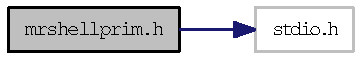
\includegraphics[width=105pt]{mrshellprim_8h__incl}
\end{center}
\end{figure}


This graph shows which files directly or indirectly include this file:\begin{figure}[H]
\begin{center}
\leavevmode
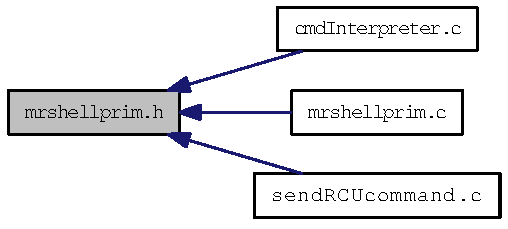
\includegraphics[width=140pt]{mrshellprim_8h__dep__incl}
\end{center}
\end{figure}
\subsection*{Data Structures}
\begin{CompactItemize}
\item 
struct \hyperlink{structTaggedData__t}{Tagged\-Data\_\-t}
\begin{CompactList}\small\item\em Named Data elements to be specified as target in an argument definition \hyperlink{structArgDef__t}{Arg\-Def\_\-t}. \item\end{CompactList}\item 
struct \hyperlink{structArgDef__t}{Arg\-Def\_\-t}
\begin{CompactList}\small\item\em The argument definition. \item\end{CompactList}\item 
struct \hyperlink{structFctMode__t}{Fct\-Mode\_\-t}
\begin{CompactList}\small\item\em Composite scan mode parameter. \item\end{CompactList}\item 
struct \hyperlink{structFctArg__t}{Fct\-Arg\_\-t}
\begin{CompactList}\small\item\em Composite parameter to specify argument definition, scan mode and an additional user pointer for type \hyperlink{mrshellprim_8h_76a810650461f2062938ee9b82666b3607fd24779fbb8e0bc12b8241e0e436cc}{e\-Fct\-Arg\-Def}. \item\end{CompactList}\end{CompactItemize}
\subsection*{Parser debugging}
\begin{CompactItemize}
\item 
\#define \hyperlink{mrshellprim_8h_9234bd75d49c86386316b90385dcd09b}{DBG\_\-SHELLPRIM\_\-MASK}~0xff0000
\begin{CompactList}\small\item\em mask for the parser debugging bits \item\end{CompactList}\item 
\#define \hyperlink{mrshellprim_8h_4831316fb2db7fbc68ce24668992227a}{DBG\_\-SEARCH\_\-ARG\_\-DEF}~0x010000
\begin{CompactList}\small\item\em debug output of the Search\-Def function \item\end{CompactList}\item 
\#define \hyperlink{mrshellprim_8h_6c6f952a74ebfbd09b41056fbd4325c0}{DBG\_\-SEARCH\_\-ARG\_\-DEF\_\-DETAIL}~0x030000
\begin{CompactList}\small\item\em detailed debug output of the Search\-Def function \item\end{CompactList}\item 
\#define \hyperlink{mrshellprim_8h_20023ac34ff79c429ae27d33b9b876ac}{DBG\_\-SCAN\_\-ARG\_\-DEF}~0x040000
\begin{CompactList}\small\item\em debug output of the Scan\-Arguments function \item\end{CompactList}\item 
\#define \hyperlink{mrshellprim_8h_166878a3f27b25b7284a00810fbd06f9}{DBG\_\-SCAN\_\-ARG\_\-DEF\_\-DETAIL}~0x0c0000
\begin{CompactList}\small\item\em detailed debug output of the Scan\-Arguments function \item\end{CompactList}\item 
\#define \hyperlink{mrshellprim_8h_6ad8cce0cc2b52f3cd9c1918405c6585}{DBG\_\-ARGUMENT\_\-READ}~0x100000
\begin{CompactList}\small\item\em debug output of the Read\-Argument function \item\end{CompactList}\item 
\#define \hyperlink{mrshellprim_8h_13095cc00efe5276cf7a1794f0f8b7e5}{DBG\_\-ARGUMENT\_\-CONVERT}~0x800000
\begin{CompactList}\small\item\em print debug information concerning argument conversion \item\end{CompactList}\item 
unsigned int \hyperlink{mrshellprim_8h_84fd8dd7e4af266b7b6a400c0cacaea4}{mr\-Shell\-Prim\-Set\-Debug\-Flag} (unsigned int flag)
\begin{CompactList}\small\item\em Set a debug flag for the parser. \item\end{CompactList}\item 
unsigned int \hyperlink{mrshellprim_8h_1d4f9511ebb635164beca6c9a4a52756}{mr\-Shell\-Prim\-Clear\-Debug\-Flag} (unsigned int flag)
\begin{CompactList}\small\item\em Clear a debug flag for the parser. \item\end{CompactList}\item 
int \hyperlink{mrshellprim_8h_20b23f294fae687b7b0ad7c6483ec564}{mr\-Shell\-Prim\-Print\-Dbg\-Flags} ()
\begin{CompactList}\small\item\em Print help information on the parser debug flags. \item\end{CompactList}\end{CompactItemize}
\subsection*{Helper functions}
\begin{CompactItemize}
\item 
\#define \hyperlink{mrshellprim_8h_3db27c9afebab8ec5e408bf1328115d0}{ARGPROC\_\-INDEX\_\-BITSHIFT}~0
\begin{CompactList}\small\item\em Result encoding for the \hyperlink{mrshellprim_8h_aa038cf5a29f51145c876af7fb5271d3}{mr\-Shell\-Prim\-Get\-Data}, \hyperlink{mrshellprim_8h_1e963c0f8d38ab1305d075b016de0a65}{mr\-Shell\-Prim\-Get\-Float}, \hyperlink{mrshellprim_8h_8f73442602070f02c40b4b3e32ab61a3}{mr\-Shell\-Prim\-Get\-Int} and \hyperlink{mrshellprim_8h_c08c7b1e961204b98f9b29120f043c6c}{mr\-Shell\-Prim\-Get\-Hex} functions. \item\end{CompactList}\item 
\#define \hyperlink{mrshellprim_8h_c69068f3119322034ba7a400e7e6d086}{ARGPROC\_\-INDEX\_\-WIDTH}~16
\begin{CompactList}\small\item\em Result encoding for the \hyperlink{mrshellprim_8h_aa038cf5a29f51145c876af7fb5271d3}{mr\-Shell\-Prim\-Get\-Data}, \hyperlink{mrshellprim_8h_1e963c0f8d38ab1305d075b016de0a65}{mr\-Shell\-Prim\-Get\-Float}, \hyperlink{mrshellprim_8h_8f73442602070f02c40b4b3e32ab61a3}{mr\-Shell\-Prim\-Get\-Int} and \hyperlink{mrshellprim_8h_c08c7b1e961204b98f9b29120f043c6c}{mr\-Shell\-Prim\-Get\-Hex} functions. \item\end{CompactList}\item 
\#define \hyperlink{mrshellprim_8h_c578c0285e80db135a272b77d4c426eb}{ARGPROC\_\-EXISTS\_\-BITSHIFT}~16
\begin{CompactList}\small\item\em Result encoding for the \hyperlink{mrshellprim_8h_aa038cf5a29f51145c876af7fb5271d3}{mr\-Shell\-Prim\-Get\-Data}, \hyperlink{mrshellprim_8h_1e963c0f8d38ab1305d075b016de0a65}{mr\-Shell\-Prim\-Get\-Float}, \hyperlink{mrshellprim_8h_8f73442602070f02c40b4b3e32ab61a3}{mr\-Shell\-Prim\-Get\-Int} and \hyperlink{mrshellprim_8h_c08c7b1e961204b98f9b29120f043c6c}{mr\-Shell\-Prim\-Get\-Hex} functions. \item\end{CompactList}\item 
\#define \hyperlink{mrshellprim_8h_8104ed49b349982ace980ced103fd593}{ARGPROC\_\-EXISTS\_\-WIDTH}~1
\begin{CompactList}\small\item\em Result encoding for the \hyperlink{mrshellprim_8h_aa038cf5a29f51145c876af7fb5271d3}{mr\-Shell\-Prim\-Get\-Data}, \hyperlink{mrshellprim_8h_1e963c0f8d38ab1305d075b016de0a65}{mr\-Shell\-Prim\-Get\-Float}, \hyperlink{mrshellprim_8h_8f73442602070f02c40b4b3e32ab61a3}{mr\-Shell\-Prim\-Get\-Int} and \hyperlink{mrshellprim_8h_c08c7b1e961204b98f9b29120f043c6c}{mr\-Shell\-Prim\-Get\-Hex} functions. \item\end{CompactList}\item 
\#define \hyperlink{mrshellprim_8h_abf55ec262e818b9d10781bbb71f18b1}{ARGPROC\_\-EXISTS}(x)~((x$>$$>$ARGPROC\_\-EXISTS\_\-BITSHIFT)\&((0x1$<$$<$ARGPROC\_\-EXISTS\_\-WIDTH)-1))
\begin{CompactList}\small\item\em helper macro to extract if the argument was found or not from the result of the \hyperlink{mrshellprim_8h_aa038cf5a29f51145c876af7fb5271d3}{mr\-Shell\-Prim\-Get\-Data}, \hyperlink{mrshellprim_8h_1e963c0f8d38ab1305d075b016de0a65}{mr\-Shell\-Prim\-Get\-Float}, \hyperlink{mrshellprim_8h_8f73442602070f02c40b4b3e32ab61a3}{mr\-Shell\-Prim\-Get\-Int} and \hyperlink{mrshellprim_8h_c08c7b1e961204b98f9b29120f043c6c}{mr\-Shell\-Prim\-Get\-Hex} functions \item\end{CompactList}\item 
\#define \hyperlink{mrshellprim_8h_4185fb7548fbc3afb73d93557631f910}{ARGPROC\_\-INDEX}(x)~((x$>$$>$ARGPROC\_\-INDEX\_\-BITSHIFT)\&((0x1$<$$<$ARGPROC\_\-INDEX\_\-WIDTH)-1))
\begin{CompactList}\small\item\em helper function to extract the index from the result of the \hyperlink{mrshellprim_8h_aa038cf5a29f51145c876af7fb5271d3}{mr\-Shell\-Prim\-Get\-Data}, \hyperlink{mrshellprim_8h_1e963c0f8d38ab1305d075b016de0a65}{mr\-Shell\-Prim\-Get\-Float}, \hyperlink{mrshellprim_8h_8f73442602070f02c40b4b3e32ab61a3}{mr\-Shell\-Prim\-Get\-Int} and \hyperlink{mrshellprim_8h_c08c7b1e961204b98f9b29120f043c6c}{mr\-Shell\-Prim\-Get\-Hex} functions \item\end{CompactList}\item 
char $\ast$ \hyperlink{mrshellprim_8h_e8ed3396fcb78ea4adce3d902b77541a}{remove\-Prec\-And\-Trailing\-Spec\-Chars} (char $\ast$p\-Cmd)
\begin{CompactList}\small\item\em Remove preceeding and trailing special characters and blanks. \item\end{CompactList}\item 
int \hyperlink{mrshellprim_8h_0244dae55f177bb00bfae3a0a39f6f5a}{get\-Hex\-Number\-From\-Arg} (const char $\ast$arg, unsigned int $\ast$p\-Number, int b\-Warning)
\begin{CompactList}\small\item\em Scan a string for a hex number. \item\end{CompactList}\item 
int \hyperlink{mrshellprim_8h_fe29afcd7e0ed24611394b379523e597}{get\-Dec\-Number\-From\-Arg} (const char $\ast$arg, int $\ast$p\-Number, int b\-Warning)
\begin{CompactList}\small\item\em Scan a string for a decimal number. \item\end{CompactList}\item 
int \hyperlink{mrshellprim_8h_bd0f88fefc2b7fb8ffa459b09018c921}{get\-Float\-Number\-From\-Arg} (const char $\ast$arg, float $\ast$p\-Number, int b\-Warning)
\begin{CompactList}\small\item\em Scan a string for a float number. \item\end{CompactList}\item 
int \hyperlink{mrshellprim_8h_cce515828d3fce502c94ea42d622bff4}{build\-Arguments\-From\-Command\-Line} (char $\ast$p\-Cmd\-Line, char $\ast$$\ast$p\-Target\-Array, int i\-Array\-Size, int b\-Separate, int i\-Debug\-Flag)
\begin{CompactList}\small\item\em Scan a buffer of characters, separate commands and extract pointers to single command parameters. \item\end{CompactList}\item 
int \hyperlink{mrshellprim_8h_24d874900c59cf760f128ae366f7a72e}{mr\-Shell\-Prim\-Get\-Index} (\hyperlink{structArgDef__t}{TArg\-Def} $\ast$array\-Def, const char $\ast$p\-Cmd, int i\-Type)
\begin{CompactList}\small\item\em Search the argument definition for a command. \item\end{CompactList}\item 
int \hyperlink{mrshellprim_8h_9f0fe9837b7198fea2f3c32bcf203ed9}{mr\-Shell\-Prim\-Set\-Data} (\hyperlink{structArgDef__t}{TArg\-Def} $\ast$array\-Def, const char $\ast$p\-Cmd, void $\ast$p\-Data, int i\-Type)
\begin{CompactList}\small\item\em Set data pointer for an argument definition element. \item\end{CompactList}\item 
int \hyperlink{mrshellprim_8h_aa038cf5a29f51145c876af7fb5271d3}{mr\-Shell\-Prim\-Get\-Data} (\hyperlink{structArgDef__t}{TArg\-Def} $\ast$array\-Def, const char $\ast$p\-Cmd, void $\ast$$\ast$pp\-Data, int i\-Type)
\begin{CompactList}\small\item\em Get data pointer for an argument definition element. \item\end{CompactList}\item 
int \hyperlink{mrshellprim_8h_1e963c0f8d38ab1305d075b016de0a65}{mr\-Shell\-Prim\-Get\-Float} (\hyperlink{structArgDef__t}{TArg\-Def} $\ast$array\-Def, const char $\ast$p\-Cmd, float $\ast$p\-Float)
\begin{CompactList}\small\item\em Get float value for an argument definition element. \item\end{CompactList}\item 
int \hyperlink{mrshellprim_8h_8f73442602070f02c40b4b3e32ab61a3}{mr\-Shell\-Prim\-Get\-Int} (\hyperlink{structArgDef__t}{TArg\-Def} $\ast$array\-Def, const char $\ast$p\-Cmd, int $\ast$p\-Int)
\begin{CompactList}\small\item\em Get integer value for an argument definition element. \item\end{CompactList}\item 
int \hyperlink{mrshellprim_8h_c08c7b1e961204b98f9b29120f043c6c}{mr\-Shell\-Prim\-Get\-Hex} (\hyperlink{structArgDef__t}{TArg\-Def} $\ast$array\-Def, const char $\ast$p\-Cmd, unsigned int $\ast$p\-Hex)
\begin{CompactList}\small\item\em Get hexadecimal value for an argument definition element. \item\end{CompactList}\item 
\hyperlink{structArgDef__t}{TArg\-Def} $\ast$ \hyperlink{mrshellprim_8h_60d2a9ecd4a849eaf72375ffeb666769}{mr\-Shell\-Prim\-Clone\-Def} (\hyperlink{structArgDef__t}{TArg\-Def} $\ast$array\-Def)
\begin{CompactList}\small\item\em Clone an argument definition. \item\end{CompactList}\item 
int \hyperlink{mrshellprim_8h_e24662763dc15a9b4719cc0f3d98f8fc}{mr\-Shell\-Prim\-Reset\-Volatile\-Flags} (\hyperlink{structArgDef__t}{TArg\-Def} $\ast$array\-Def)
\begin{CompactList}\small\item\em Reset volatile processing flags of the definition array. \item\end{CompactList}\end{CompactItemize}
\subsection*{Defines}
\begin{CompactItemize}
\item 
\#define \hyperlink{mrshellprim_8h_86460f91fb298845d3b49c21b3a8a420}{SCANMODE\_\-STRICT\_\-SEQUENCE}~0x0001
\begin{CompactList}\small\item\em require the sequence of all mandatory arguments \item\end{CompactList}\item 
\#define \hyperlink{mrshellprim_8h_3c911f1397ec09fbcc6a1feac53be850}{SCANMODE\_\-FORCE\_\-TERMINATION}~0x0002
\begin{CompactList}\small\item\em terminate at the first not-recognized argument \item\end{CompactList}\item 
\#define \hyperlink{mrshellprim_8h_c2d1f169c5bb97507a98cda7ce973332}{SCANMODE\_\-PRINT\_\-UKWN\_\-SEQU}~0x0004
\begin{CompactList}\small\item\em write an unknown sequence to the output \item\end{CompactList}\item 
\#define \hyperlink{mrshellprim_8h_44108151eef216f1bbe017e9e1503c50}{SCANMODE\_\-SILENT}~0x0008
\begin{CompactList}\small\item\em dont report an error in case of unknown argument \item\end{CompactList}\item 
\#define \hyperlink{mrshellprim_8h_65e7fef3ff265436f120f3b3c070aff0}{SCANMODE\_\-SKIP\_\-UKWN\_\-SEQU}~0x0010
\begin{CompactList}\small\item\em skip an unknown sequence and continue \item\end{CompactList}\item 
\#define \hyperlink{mrshellprim_8h_b41f1fbe57be88462133d6065f48a9f9}{SCANMODE\_\-READ\_\-ONE\_\-CMD}~0x0020
\begin{CompactList}\small\item\em read only one command with all the arguments and terminate \item\end{CompactList}\item 
\#define \hyperlink{mrshellprim_8h_222a83d015679c34e763bc9f7d9778c5}{SCANMODE\_\-PERSISTENT}~0x0040
\begin{CompactList}\small\item\em do not clean volatile flags at the beginning of the argument scan \item\end{CompactList}\item 
\#define \hyperlink{mrshellprim_8h_8c595e09c68cb8c5ca0ce78002f48caf}{SCANRET\_\-BITSHIFT\_\-PROCESSED\_\-ARGS}~8
\item 
\#define \hyperlink{mrshellprim_8h_720b462066770425625df7cbf09e2274}{SCANRET\_\-BITSHIFT\_\-OFFSET\_\-LAST\_\-ARG}~0
\item 
\#define \hyperlink{mrshellprim_8h_9402133885fb87b81c4835a8fa4d7111}{SCANRET\_\-BITSHIFT\_\-INDEX}~16
\item 
\#define \hyperlink{mrshellprim_8h_26c19cdba298002712c08c9964edd0df}{SCANRET\_\-MASK\_\-PROCESSED\_\-ARGS}~0x0000ff00
\item 
\#define \hyperlink{mrshellprim_8h_b17dfbdaa414a0479199510989ed3daf}{SCANRET\_\-MASK\_\-OFFSET\_\-LAST\_\-ARG}~0x000000ff
\item 
\#define \hyperlink{mrshellprim_8h_37fb2e6805fb0fc8a1a19cf7b75b2a54}{SCANRET\_\-MASK\_\-INDEX}~0x00ff0000
\item 
\#define \hyperlink{mrshellprim_8h_660c0a7279105aabf7af9b5305d10edd}{SCANRET\_\-INVAL\_\-INDEX}~0x000000ff
\item 
\#define \hyperlink{mrshellprim_8h_fac0d386803ac2c52587855f31847135}{SCANRET\_\-GET\_\-PROCESSED\_\-ARGS}~((x\&SCANRET\_\-MASK\_\-PROCESSED\_\-ARGS)$>$$>$SCANRET\_\-BITSHIFT\_\-PROCESSED\_\-ARGS)
\item 
\#define \hyperlink{mrshellprim_8h_b88030964c6af549b6d439d7247b55ae}{SCANRET\_\-GET\_\-OFFSET\_\-LAST\_\-ARG}~((x\&SCANRET\_\-MASK\_\-OFFSET\_\-LAST\_\-ARG)$>$$>$SCANRET\_\-BITSHIFT\_\-OFFSET\_\-LAST\_\-ARG)
\item 
\#define \hyperlink{mrshellprim_8h_7575098e36ae87b0e09ca0134111771b}{ARGDEF\_\-MANDATORY}~0x0001
\begin{CompactList}\small\item\em mark the argument as mandatory \item\end{CompactList}\item 
\#define \hyperlink{mrshellprim_8h_e0eafe007ee0938f2fa284de82b5a423}{ARGDEF\_\-OPTIONAL}~0x0002
\begin{CompactList}\small\item\em mark the argument as optional \item\end{CompactList}\item 
\#define \hyperlink{mrshellprim_8h_88a540f6af1088e73e5a2c6f7070387c}{ARGDEF\_\-ONLY\_\-ONCE}~0x0004
\begin{CompactList}\small\item\em the argument will be ignored for further check if read once \item\end{CompactList}\item 
\#define \hyperlink{mrshellprim_8h_3cc896907567bba4ccba5583d28c382a}{ARGDEF\_\-SKIP\_\-IF\_\-FAILED}~0x0008
\begin{CompactList}\small\item\em skip the argument if the required additional argument scan failed \item\end{CompactList}\item 
\#define \hyperlink{mrshellprim_8h_c02c4c51c3c6ef7eddc4bd49a0f8df75}{ARGDEF\_\-RESUME}~0x0010
\begin{CompactList}\small\item\em if additional scans fail resume and try to find another entry in the definition array \item\end{CompactList}\item 
\#define \hyperlink{mrshellprim_8h_6ec4b88030cc16c92c86aa9fcd1789ee}{ARGDEF\_\-UNTERM\_\-SHORT}~0x0020
\begin{CompactList}\small\item\em the short argument does not need to be terminated by a separator \item\end{CompactList}\item 
\#define \hyperlink{mrshellprim_8h_9ecb4288871a72cb5f4cb8428498de9c}{ARGDEF\_\-UNTERM\_\-LONG}~0x0040
\begin{CompactList}\small\item\em the long argument does not need to be terminated by a separator \item\end{CompactList}\item 
\#define \hyperlink{mrshellprim_8h_ba7cfe65a42313488b4cfdf335409d39}{ARGDEF\_\-TERMINATE}~0x0080
\begin{CompactList}\small\item\em terminate the argument scan after this argument was processed \item\end{CompactList}\item 
\#define \hyperlink{mrshellprim_8h_418c1127f3854b9a10562114b5ca73d8}{ARGDEF\_\-EXIT}~0x0100
\begin{CompactList}\small\item\em terminate without processing with -EINTR if this argument was found \item\end{CompactList}\item 
\#define \hyperlink{mrshellprim_8h_fc218ec9b386341226b551419f3f624c}{ARGDEF\_\-BREAK}~0x0200
\begin{CompactList}\small\item\em terminate without processing if this argument was found \item\end{CompactList}\item 
\#define \hyperlink{mrshellprim_8h_bbe395069287967226d76ca691690f6a}{ARGDEF\_\-DELAY\_\-EXECUTE}~0x0400
\begin{CompactList}\small\item\em dont call subfunctions for this argument definition \item\end{CompactList}\item 
\#define \hyperlink{mrshellprim_8h_9f63a516fdf6cc051373d525521dd03b}{ARGDEF\_\-KEYWORDLESS}~0x0800
\begin{CompactList}\small\item\em this is a keywordless argument, start scanning the parameters from the argument itself \item\end{CompactList}\end{CompactItemize}
\subsection*{Typedefs}
\begin{CompactItemize}
\item 
typedef \hyperlink{structArgDef__t}{Arg\-Def\_\-t} \hyperlink{mrshellprim_8h_29dc127323f25100255dd42e412fafc4}{TArg\-Def}
\begin{CompactList}\small\item\em Type define for the argument definition structure. \item\end{CompactList}\item 
typedef \hyperlink{structFctMode__t}{Fct\-Mode\_\-t} \hyperlink{mrshellprim_8h_20221874fc8a934770e163918e7a8125}{TFct\-Mode}
\begin{CompactList}\small\item\em Type define for the function mode structure. \item\end{CompactList}\item 
typedef \hyperlink{structFctArg__t}{Fct\-Arg\_\-t} \hyperlink{mrshellprim_8h_7d991941e20cbebfb3b65a18e6f17f20}{TFct\-Arg}
\begin{CompactList}\small\item\em Type define for the function arg structure. \item\end{CompactList}\item 
typedef \hyperlink{structTaggedData__t}{Tagged\-Data\_\-t} \hyperlink{mrshellprim_8h_8523df93cf35a7060519eac48ad6def6}{TTagged\-Data}
\begin{CompactList}\small\item\em Type define for the tagged data structure. \item\end{CompactList}\item 
typedef int($\ast$) \hyperlink{mrshellprim_8h_25a848858601a9d7593db26db1933c8f}{Function\-No\-Arg} ()
\begin{CompactList}\small\item\em Type define for a processing function with no arguments. \item\end{CompactList}\item 
typedef int($\ast$) \hyperlink{mrshellprim_8h_13b0972f6d0c45d484e999ced9aa622c}{Fct\-Index} (int major\-No)
\begin{CompactList}\small\item\em Type define for a processing function with an int index argument. \item\end{CompactList}\item 
typedef int($\ast$) \hyperlink{mrshellprim_8h_8f5e79dc67d35c6c5990f753f9490708}{Fct\-User\-Scan} (const char $\ast$current\-Arg, const char $\ast$$\ast$array\-Arg, int i\-Nof\-Args, void $\ast$p\-User, FILE $\ast$p\-Out)
\begin{CompactList}\small\item\em Type define for a user defined scan function. \item\end{CompactList}\item 
typedef int($\ast$) \hyperlink{mrshellprim_8h_6dfb2d9a1efb85cb44f59123ebdb1cc4}{Fct\-Integer} (int $\ast$array, int i\-Nof\-Args, FILE $\ast$p\-Out)
\begin{CompactList}\small\item\em Type define for a processing function with an integer array argument. \item\end{CompactList}\item 
typedef int($\ast$) \hyperlink{mrshellprim_8h_027c8c25e67dc4b7346ac5713cf673ab}{Fct\-Float} (float $\ast$array, int i\-Nof\-Args, FILE $\ast$p\-Out)
\begin{CompactList}\small\item\em Type define for a processing function with a float array argument. \item\end{CompactList}\item 
typedef int($\ast$) \hyperlink{mrshellprim_8h_7e40ba8c9e984665cfe0dbd2b4fa888a}{Fct\-Hex} (unsigned long $\ast$array, int i\-Nof\-Args, FILE $\ast$p\-Out)
\begin{CompactList}\small\item\em Type define for a processing function with a hex array argument. \item\end{CompactList}\item 
typedef int($\ast$) \hyperlink{mrshellprim_8h_fdf1e7a245d5ec6ac61d531e07e6a33c}{Fct\-Composite} (\hyperlink{structTaggedData__t}{TTagged\-Data} $\ast$array, int i\-Nof\-Args, FILE $\ast$p\-Out)
\begin{CompactList}\small\item\em Type define for a processing function with a composite array argument. \item\end{CompactList}\item 
typedef int($\ast$) \hyperlink{mrshellprim_8h_1c9f7567aaf5693ef8473ff91ccb8ff5}{Fct\-Arg\-Def} (\hyperlink{structArgDef__t}{TArg\-Def} $\ast$p\-Def, void $\ast$p\-User, FILE $\ast$p\-Out)
\begin{CompactList}\small\item\em Type define for a processing function for a successful argument scan. \item\end{CompactList}\end{CompactItemize}
\subsection*{Enumerations}
\begin{CompactItemize}
\item 
enum \hyperlink{mrshellprim_8h_76a810650461f2062938ee9b82666b36}{operation\_\-t} \{ \par
\hyperlink{mrshellprim_8h_76a810650461f2062938ee9b82666b36a94b1781ada88507c56c4475f25fa92f}{e\-Unknown\-Type} =  0, 
\hyperlink{mrshellprim_8h_76a810650461f2062938ee9b82666b36dd647739976fe8f17c25e3fe04d30eeb}{e\-Integer}, 
\hyperlink{mrshellprim_8h_76a810650461f2062938ee9b82666b36f56ebbf9f6232a573f846cffa9f914e9}{e\-Integer\-Array}, 
\hyperlink{mrshellprim_8h_76a810650461f2062938ee9b82666b364a5cba5eee27b47a9cf3714e4db4206d}{e\-Float}, 
\par
\hyperlink{mrshellprim_8h_76a810650461f2062938ee9b82666b361cf54b260432a1baf68bed16081357c7}{e\-Float\-Array}, 
\hyperlink{mrshellprim_8h_76a810650461f2062938ee9b82666b36a64d04be3dc94180a329fac904a5d239}{e\-Hex}, 
\hyperlink{mrshellprim_8h_76a810650461f2062938ee9b82666b36be303c42da892f2d0101b668e8aa252a}{e\-Hex\-Array}, 
\hyperlink{mrshellprim_8h_76a810650461f2062938ee9b82666b369bf242e7bb183d9518928958c83c9a22}{e\-Const\-String}, 
\par
\hyperlink{mrshellprim_8h_76a810650461f2062938ee9b82666b360a10a6c7f681516162b85d6096fc394e}{e\-Char\-Array}, 
\hyperlink{mrshellprim_8h_76a810650461f2062938ee9b82666b36da4dfcdd447a4ba250c0f9b7c2dbf21e}{e\-Composite}, 
\hyperlink{mrshellprim_8h_76a810650461f2062938ee9b82666b3693da28770e1bd5abcff3bfab36328f85}{e\-Fct\-No\-Arg}, 
\hyperlink{mrshellprim_8h_76a810650461f2062938ee9b82666b369d37de9621433ecd8d0b29cb7a8b1536}{e\-Fct\-Index}, 
\par
\hyperlink{mrshellprim_8h_76a810650461f2062938ee9b82666b36b36d09249e94b5aa513d0aa3c7aa08c8}{e\-Fct\-Remaining}, 
\hyperlink{mrshellprim_8h_76a810650461f2062938ee9b82666b364c15eefaf9247f7b503ae586294be587}{e\-Fct\-Inclusive}, 
\hyperlink{mrshellprim_8h_76a810650461f2062938ee9b82666b36b17c2f574c8a5697b118c8aa4a00bdad}{e\-Fct\-User\-Scan}, 
\hyperlink{mrshellprim_8h_76a810650461f2062938ee9b82666b366feb19b8074a5ad5e422022891e6e2f5}{e\-Fct\-Integer\-Args}, 
\par
\hyperlink{mrshellprim_8h_76a810650461f2062938ee9b82666b363cf1e6253af3a5870b9c8cc15ce25900}{e\-Fct\-Float\-Args}, 
\hyperlink{mrshellprim_8h_76a810650461f2062938ee9b82666b3654420a8008623d27ad4e6cf8ba76f7b8}{e\-Fct\-Hex\-Args}, 
\hyperlink{mrshellprim_8h_76a810650461f2062938ee9b82666b3636b7e40fa597a694a95e617ee33e0e6b}{e\-Fct\-Composite\-Args}, 
\hyperlink{mrshellprim_8h_76a810650461f2062938ee9b82666b3607fd24779fbb8e0bc12b8241e0e436cc}{e\-Fct\-Arg\-Def}, 
\par
\hyperlink{mrshellprim_8h_76a810650461f2062938ee9b82666b365461a9e2704387e11258e14a0b41ac1a}{e\-Bool}, 
\hyperlink{mrshellprim_8h_76a810650461f2062938ee9b82666b36514baa0f6ca7bbfba804b8826c13cffb}{e\-Flag}
 \}
\begin{CompactList}\small\item\em The operation identifiers. \item\end{CompactList}\end{CompactItemize}
\subsection*{Functions}
\begin{CompactItemize}
\item 
int \hyperlink{mrshellprim_8h_e2735ecedc52b1199ecf8a208339c072}{Scan\-Arguments} (const char $\ast$$\ast$array\-Arg, int i\-Nof\-Args, int i\-First\-Arg\-Start, \hyperlink{structArgDef__t}{TArg\-Def} $\ast$array\-Def, \hyperlink{structFctMode__t}{TFct\-Mode} $\ast$p\-Mode)
\begin{CompactList}\small\item\em Scan a list or single string of arguments. \item\end{CompactList}\item 
int \hyperlink{mrshellprim_8h_d50cc0ad50efa63a876cee5ef7caed9f}{Print\-Argument\-Definition} (\hyperlink{structArgDef__t}{TArg\-Def} $\ast$array\-Def, int b\-All)
\begin{CompactList}\small\item\em Print a summury on the argument definition structure. \item\end{CompactList}\end{CompactItemize}


\subsection{Detailed Description}
A command line parser. 

\begin{Desc}
\item[Author:]Matthias Richter \end{Desc}


Definition in file \hyperlink{mrshellprim_8h-source}{mrshellprim.h}.

\subsection{Define Documentation}
\hypertarget{mrshellprim_8h_fc218ec9b386341226b551419f3f624c}{
\index{mrshellprim.h@{mrshellprim.h}!ARGDEF_BREAK@{ARGDEF\_\-BREAK}}
\index{ARGDEF_BREAK@{ARGDEF\_\-BREAK}!mrshellprim.h@{mrshellprim.h}}
\subsubsection[ARGDEF\_\-BREAK]{\setlength{\rightskip}{0pt plus 5cm}\#define ARGDEF\_\-BREAK~0x0200}}
\label{mrshellprim_8h_fc218ec9b386341226b551419f3f624c}


terminate without processing if this argument was found 



Definition at line 224 of file mrshellprim.h.

Referenced by Scan\-Arguments().\hypertarget{mrshellprim_8h_bbe395069287967226d76ca691690f6a}{
\index{mrshellprim.h@{mrshellprim.h}!ARGDEF_DELAY_EXECUTE@{ARGDEF\_\-DELAY\_\-EXECUTE}}
\index{ARGDEF_DELAY_EXECUTE@{ARGDEF\_\-DELAY\_\-EXECUTE}!mrshellprim.h@{mrshellprim.h}}
\subsubsection[ARGDEF\_\-DELAY\_\-EXECUTE]{\setlength{\rightskip}{0pt plus 5cm}\#define ARGDEF\_\-DELAY\_\-EXECUTE~0x0400}}
\label{mrshellprim_8h_bbe395069287967226d76ca691690f6a}


dont call subfunctions for this argument definition 



Definition at line 226 of file mrshellprim.h.

Referenced by Scan\-Arguments().\hypertarget{mrshellprim_8h_418c1127f3854b9a10562114b5ca73d8}{
\index{mrshellprim.h@{mrshellprim.h}!ARGDEF_EXIT@{ARGDEF\_\-EXIT}}
\index{ARGDEF_EXIT@{ARGDEF\_\-EXIT}!mrshellprim.h@{mrshellprim.h}}
\subsubsection[ARGDEF\_\-EXIT]{\setlength{\rightskip}{0pt plus 5cm}\#define ARGDEF\_\-EXIT~0x0100}}
\label{mrshellprim_8h_418c1127f3854b9a10562114b5ca73d8}


terminate without processing with -EINTR if this argument was found 



Definition at line 222 of file mrshellprim.h.

Referenced by Scan\-Arguments().\hypertarget{mrshellprim_8h_9f63a516fdf6cc051373d525521dd03b}{
\index{mrshellprim.h@{mrshellprim.h}!ARGDEF_KEYWORDLESS@{ARGDEF\_\-KEYWORDLESS}}
\index{ARGDEF_KEYWORDLESS@{ARGDEF\_\-KEYWORDLESS}!mrshellprim.h@{mrshellprim.h}}
\subsubsection[ARGDEF\_\-KEYWORDLESS]{\setlength{\rightskip}{0pt plus 5cm}\#define ARGDEF\_\-KEYWORDLESS~0x0800}}
\label{mrshellprim_8h_9f63a516fdf6cc051373d525521dd03b}


this is a keywordless argument, start scanning the parameters from the argument itself 



Definition at line 228 of file mrshellprim.h.

Referenced by Search\-Def().\hypertarget{mrshellprim_8h_7575098e36ae87b0e09ca0134111771b}{
\index{mrshellprim.h@{mrshellprim.h}!ARGDEF_MANDATORY@{ARGDEF\_\-MANDATORY}}
\index{ARGDEF_MANDATORY@{ARGDEF\_\-MANDATORY}!mrshellprim.h@{mrshellprim.h}}
\subsubsection[ARGDEF\_\-MANDATORY]{\setlength{\rightskip}{0pt plus 5cm}\#define ARGDEF\_\-MANDATORY~0x0001}}
\label{mrshellprim_8h_7575098e36ae87b0e09ca0134111771b}


mark the argument as mandatory 



Definition at line 206 of file mrshellprim.h.\hypertarget{mrshellprim_8h_88a540f6af1088e73e5a2c6f7070387c}{
\index{mrshellprim.h@{mrshellprim.h}!ARGDEF_ONLY_ONCE@{ARGDEF\_\-ONLY\_\-ONCE}}
\index{ARGDEF_ONLY_ONCE@{ARGDEF\_\-ONLY\_\-ONCE}!mrshellprim.h@{mrshellprim.h}}
\subsubsection[ARGDEF\_\-ONLY\_\-ONCE]{\setlength{\rightskip}{0pt plus 5cm}\#define ARGDEF\_\-ONLY\_\-ONCE~0x0004}}
\label{mrshellprim_8h_88a540f6af1088e73e5a2c6f7070387c}


the argument will be ignored for further check if read once 



Definition at line 210 of file mrshellprim.h.

Referenced by Search\-Def().\hypertarget{mrshellprim_8h_e0eafe007ee0938f2fa284de82b5a423}{
\index{mrshellprim.h@{mrshellprim.h}!ARGDEF_OPTIONAL@{ARGDEF\_\-OPTIONAL}}
\index{ARGDEF_OPTIONAL@{ARGDEF\_\-OPTIONAL}!mrshellprim.h@{mrshellprim.h}}
\subsubsection[ARGDEF\_\-OPTIONAL]{\setlength{\rightskip}{0pt plus 5cm}\#define ARGDEF\_\-OPTIONAL~0x0002}}
\label{mrshellprim_8h_e0eafe007ee0938f2fa284de82b5a423}


mark the argument as optional 



Definition at line 208 of file mrshellprim.h.\hypertarget{mrshellprim_8h_c02c4c51c3c6ef7eddc4bd49a0f8df75}{
\index{mrshellprim.h@{mrshellprim.h}!ARGDEF_RESUME@{ARGDEF\_\-RESUME}}
\index{ARGDEF_RESUME@{ARGDEF\_\-RESUME}!mrshellprim.h@{mrshellprim.h}}
\subsubsection[ARGDEF\_\-RESUME]{\setlength{\rightskip}{0pt plus 5cm}\#define ARGDEF\_\-RESUME~0x0010}}
\label{mrshellprim_8h_c02c4c51c3c6ef7eddc4bd49a0f8df75}


if additional scans fail resume and try to find another entry in the definition array 



Definition at line 214 of file mrshellprim.h.

Referenced by Scan\-Arguments().\hypertarget{mrshellprim_8h_3cc896907567bba4ccba5583d28c382a}{
\index{mrshellprim.h@{mrshellprim.h}!ARGDEF_SKIP_IF_FAILED@{ARGDEF\_\-SKIP\_\-IF\_\-FAILED}}
\index{ARGDEF_SKIP_IF_FAILED@{ARGDEF\_\-SKIP\_\-IF\_\-FAILED}!mrshellprim.h@{mrshellprim.h}}
\subsubsection[ARGDEF\_\-SKIP\_\-IF\_\-FAILED]{\setlength{\rightskip}{0pt plus 5cm}\#define ARGDEF\_\-SKIP\_\-IF\_\-FAILED~0x0008}}
\label{mrshellprim_8h_3cc896907567bba4ccba5583d28c382a}


skip the argument if the required additional argument scan failed 



Definition at line 212 of file mrshellprim.h.\hypertarget{mrshellprim_8h_ba7cfe65a42313488b4cfdf335409d39}{
\index{mrshellprim.h@{mrshellprim.h}!ARGDEF_TERMINATE@{ARGDEF\_\-TERMINATE}}
\index{ARGDEF_TERMINATE@{ARGDEF\_\-TERMINATE}!mrshellprim.h@{mrshellprim.h}}
\subsubsection[ARGDEF\_\-TERMINATE]{\setlength{\rightskip}{0pt plus 5cm}\#define ARGDEF\_\-TERMINATE~0x0080}}
\label{mrshellprim_8h_ba7cfe65a42313488b4cfdf335409d39}


terminate the argument scan after this argument was processed 



Definition at line 220 of file mrshellprim.h.

Referenced by Scan\-Arguments().\hypertarget{mrshellprim_8h_9ecb4288871a72cb5f4cb8428498de9c}{
\index{mrshellprim.h@{mrshellprim.h}!ARGDEF_UNTERM_LONG@{ARGDEF\_\-UNTERM\_\-LONG}}
\index{ARGDEF_UNTERM_LONG@{ARGDEF\_\-UNTERM\_\-LONG}!mrshellprim.h@{mrshellprim.h}}
\subsubsection[ARGDEF\_\-UNTERM\_\-LONG]{\setlength{\rightskip}{0pt plus 5cm}\#define ARGDEF\_\-UNTERM\_\-LONG~0x0040}}
\label{mrshellprim_8h_9ecb4288871a72cb5f4cb8428498de9c}


the long argument does not need to be terminated by a separator 



Definition at line 218 of file mrshellprim.h.

Referenced by Search\-Def().\hypertarget{mrshellprim_8h_6ec4b88030cc16c92c86aa9fcd1789ee}{
\index{mrshellprim.h@{mrshellprim.h}!ARGDEF_UNTERM_SHORT@{ARGDEF\_\-UNTERM\_\-SHORT}}
\index{ARGDEF_UNTERM_SHORT@{ARGDEF\_\-UNTERM\_\-SHORT}!mrshellprim.h@{mrshellprim.h}}
\subsubsection[ARGDEF\_\-UNTERM\_\-SHORT]{\setlength{\rightskip}{0pt plus 5cm}\#define ARGDEF\_\-UNTERM\_\-SHORT~0x0020}}
\label{mrshellprim_8h_6ec4b88030cc16c92c86aa9fcd1789ee}


the short argument does not need to be terminated by a separator 



Definition at line 216 of file mrshellprim.h.

Referenced by Search\-Def().\hypertarget{mrshellprim_8h_abf55ec262e818b9d10781bbb71f18b1}{
\index{mrshellprim.h@{mrshellprim.h}!ARGPROC_EXISTS@{ARGPROC\_\-EXISTS}}
\index{ARGPROC_EXISTS@{ARGPROC\_\-EXISTS}!mrshellprim.h@{mrshellprim.h}}
\subsubsection[ARGPROC\_\-EXISTS]{\setlength{\rightskip}{0pt plus 5cm}\#define ARGPROC\_\-EXISTS(x)~((x$>$$>$ARGPROC\_\-EXISTS\_\-BITSHIFT)\&((0x1$<$$<$ARGPROC\_\-EXISTS\_\-WIDTH)-1))}}
\label{mrshellprim_8h_abf55ec262e818b9d10781bbb71f18b1}


helper macro to extract if the argument was found or not from the result of the \hyperlink{mrshellprim_8h_aa038cf5a29f51145c876af7fb5271d3}{mr\-Shell\-Prim\-Get\-Data}, \hyperlink{mrshellprim_8h_1e963c0f8d38ab1305d075b016de0a65}{mr\-Shell\-Prim\-Get\-Float}, \hyperlink{mrshellprim_8h_8f73442602070f02c40b4b3e32ab61a3}{mr\-Shell\-Prim\-Get\-Int} and \hyperlink{mrshellprim_8h_c08c7b1e961204b98f9b29120f043c6c}{mr\-Shell\-Prim\-Get\-Hex} functions 



Definition at line 592 of file mrshellprim.h.

Referenced by driver\-Ctrl\-Cmds(), exec\-Flash\-Erase(), and main().\hypertarget{mrshellprim_8h_c578c0285e80db135a272b77d4c426eb}{
\index{mrshellprim.h@{mrshellprim.h}!ARGPROC_EXISTS_BITSHIFT@{ARGPROC\_\-EXISTS\_\-BITSHIFT}}
\index{ARGPROC_EXISTS_BITSHIFT@{ARGPROC\_\-EXISTS\_\-BITSHIFT}!mrshellprim.h@{mrshellprim.h}}
\subsubsection[ARGPROC\_\-EXISTS\_\-BITSHIFT]{\setlength{\rightskip}{0pt plus 5cm}\#define ARGPROC\_\-EXISTS\_\-BITSHIFT~16}}
\label{mrshellprim_8h_c578c0285e80db135a272b77d4c426eb}


Result encoding for the \hyperlink{mrshellprim_8h_aa038cf5a29f51145c876af7fb5271d3}{mr\-Shell\-Prim\-Get\-Data}, \hyperlink{mrshellprim_8h_1e963c0f8d38ab1305d075b016de0a65}{mr\-Shell\-Prim\-Get\-Float}, \hyperlink{mrshellprim_8h_8f73442602070f02c40b4b3e32ab61a3}{mr\-Shell\-Prim\-Get\-Int} and \hyperlink{mrshellprim_8h_c08c7b1e961204b98f9b29120f043c6c}{mr\-Shell\-Prim\-Get\-Hex} functions. 



Definition at line 581 of file mrshellprim.h.

Referenced by mr\-Shell\-Prim\-Get\-Data(), mr\-Shell\-Prim\-Get\-Float(), mr\-Shell\-Prim\-Get\-Hex(), and mr\-Shell\-Prim\-Get\-Int().\hypertarget{mrshellprim_8h_8104ed49b349982ace980ced103fd593}{
\index{mrshellprim.h@{mrshellprim.h}!ARGPROC_EXISTS_WIDTH@{ARGPROC\_\-EXISTS\_\-WIDTH}}
\index{ARGPROC_EXISTS_WIDTH@{ARGPROC\_\-EXISTS\_\-WIDTH}!mrshellprim.h@{mrshellprim.h}}
\subsubsection[ARGPROC\_\-EXISTS\_\-WIDTH]{\setlength{\rightskip}{0pt plus 5cm}\#define ARGPROC\_\-EXISTS\_\-WIDTH~1}}
\label{mrshellprim_8h_8104ed49b349982ace980ced103fd593}


Result encoding for the \hyperlink{mrshellprim_8h_aa038cf5a29f51145c876af7fb5271d3}{mr\-Shell\-Prim\-Get\-Data}, \hyperlink{mrshellprim_8h_1e963c0f8d38ab1305d075b016de0a65}{mr\-Shell\-Prim\-Get\-Float}, \hyperlink{mrshellprim_8h_8f73442602070f02c40b4b3e32ab61a3}{mr\-Shell\-Prim\-Get\-Int} and \hyperlink{mrshellprim_8h_c08c7b1e961204b98f9b29120f043c6c}{mr\-Shell\-Prim\-Get\-Hex} functions. 



Definition at line 586 of file mrshellprim.h.\hypertarget{mrshellprim_8h_4185fb7548fbc3afb73d93557631f910}{
\index{mrshellprim.h@{mrshellprim.h}!ARGPROC_INDEX@{ARGPROC\_\-INDEX}}
\index{ARGPROC_INDEX@{ARGPROC\_\-INDEX}!mrshellprim.h@{mrshellprim.h}}
\subsubsection[ARGPROC\_\-INDEX]{\setlength{\rightskip}{0pt plus 5cm}\#define ARGPROC\_\-INDEX(x)~((x$>$$>$ARGPROC\_\-INDEX\_\-BITSHIFT)\&((0x1$<$$<$ARGPROC\_\-INDEX\_\-WIDTH)-1))}}
\label{mrshellprim_8h_4185fb7548fbc3afb73d93557631f910}


helper function to extract the index from the result of the \hyperlink{mrshellprim_8h_aa038cf5a29f51145c876af7fb5271d3}{mr\-Shell\-Prim\-Get\-Data}, \hyperlink{mrshellprim_8h_1e963c0f8d38ab1305d075b016de0a65}{mr\-Shell\-Prim\-Get\-Float}, \hyperlink{mrshellprim_8h_8f73442602070f02c40b4b3e32ab61a3}{mr\-Shell\-Prim\-Get\-Int} and \hyperlink{mrshellprim_8h_c08c7b1e961204b98f9b29120f043c6c}{mr\-Shell\-Prim\-Get\-Hex} functions 



Definition at line 598 of file mrshellprim.h.\hypertarget{mrshellprim_8h_3db27c9afebab8ec5e408bf1328115d0}{
\index{mrshellprim.h@{mrshellprim.h}!ARGPROC_INDEX_BITSHIFT@{ARGPROC\_\-INDEX\_\-BITSHIFT}}
\index{ARGPROC_INDEX_BITSHIFT@{ARGPROC\_\-INDEX\_\-BITSHIFT}!mrshellprim.h@{mrshellprim.h}}
\subsubsection[ARGPROC\_\-INDEX\_\-BITSHIFT]{\setlength{\rightskip}{0pt plus 5cm}\#define ARGPROC\_\-INDEX\_\-BITSHIFT~0}}
\label{mrshellprim_8h_3db27c9afebab8ec5e408bf1328115d0}


Result encoding for the \hyperlink{mrshellprim_8h_aa038cf5a29f51145c876af7fb5271d3}{mr\-Shell\-Prim\-Get\-Data}, \hyperlink{mrshellprim_8h_1e963c0f8d38ab1305d075b016de0a65}{mr\-Shell\-Prim\-Get\-Float}, \hyperlink{mrshellprim_8h_8f73442602070f02c40b4b3e32ab61a3}{mr\-Shell\-Prim\-Get\-Int} and \hyperlink{mrshellprim_8h_c08c7b1e961204b98f9b29120f043c6c}{mr\-Shell\-Prim\-Get\-Hex} functions. 



Definition at line 571 of file mrshellprim.h.\hypertarget{mrshellprim_8h_c69068f3119322034ba7a400e7e6d086}{
\index{mrshellprim.h@{mrshellprim.h}!ARGPROC_INDEX_WIDTH@{ARGPROC\_\-INDEX\_\-WIDTH}}
\index{ARGPROC_INDEX_WIDTH@{ARGPROC\_\-INDEX\_\-WIDTH}!mrshellprim.h@{mrshellprim.h}}
\subsubsection[ARGPROC\_\-INDEX\_\-WIDTH]{\setlength{\rightskip}{0pt plus 5cm}\#define ARGPROC\_\-INDEX\_\-WIDTH~16}}
\label{mrshellprim_8h_c69068f3119322034ba7a400e7e6d086}


Result encoding for the \hyperlink{mrshellprim_8h_aa038cf5a29f51145c876af7fb5271d3}{mr\-Shell\-Prim\-Get\-Data}, \hyperlink{mrshellprim_8h_1e963c0f8d38ab1305d075b016de0a65}{mr\-Shell\-Prim\-Get\-Float}, \hyperlink{mrshellprim_8h_8f73442602070f02c40b4b3e32ab61a3}{mr\-Shell\-Prim\-Get\-Int} and \hyperlink{mrshellprim_8h_c08c7b1e961204b98f9b29120f043c6c}{mr\-Shell\-Prim\-Get\-Hex} functions. 



Definition at line 576 of file mrshellprim.h.\hypertarget{mrshellprim_8h_13095cc00efe5276cf7a1794f0f8b7e5}{
\index{mrshellprim.h@{mrshellprim.h}!DBG_ARGUMENT_CONVERT@{DBG\_\-ARGUMENT\_\-CONVERT}}
\index{DBG_ARGUMENT_CONVERT@{DBG\_\-ARGUMENT\_\-CONVERT}!mrshellprim.h@{mrshellprim.h}}
\subsubsection[DBG\_\-ARGUMENT\_\-CONVERT]{\setlength{\rightskip}{0pt plus 5cm}\#define DBG\_\-ARGUMENT\_\-CONVERT~0x800000}}
\label{mrshellprim_8h_13095cc00efe5276cf7a1794f0f8b7e5}


print debug information concerning argument conversion 



Definition at line 381 of file mrshellprim.h.

Referenced by build\-Arguments\-From\-Command\-Line(), execute\-Command\-Line(), execute\-Main\-Commands(), mr\-Shell\-Prim\-Print\-Dbg\-Flags(), print\-Debug\-Help(), print\-Read\-Output\-Formatted(), Scan\-Coefficients(), and wait\-Condition().\hypertarget{mrshellprim_8h_6ad8cce0cc2b52f3cd9c1918405c6585}{
\index{mrshellprim.h@{mrshellprim.h}!DBG_ARGUMENT_READ@{DBG\_\-ARGUMENT\_\-READ}}
\index{DBG_ARGUMENT_READ@{DBG\_\-ARGUMENT\_\-READ}!mrshellprim.h@{mrshellprim.h}}
\subsubsection[DBG\_\-ARGUMENT\_\-READ]{\setlength{\rightskip}{0pt plus 5cm}\#define DBG\_\-ARGUMENT\_\-READ~0x100000}}
\label{mrshellprim_8h_6ad8cce0cc2b52f3cd9c1918405c6585}


debug output of the Read\-Argument function 



Definition at line 379 of file mrshellprim.h.

Referenced by mr\-Shell\-Prim\-Print\-Dbg\-Flags(), and Read\-Argument().\hypertarget{mrshellprim_8h_20023ac34ff79c429ae27d33b9b876ac}{
\index{mrshellprim.h@{mrshellprim.h}!DBG_SCAN_ARG_DEF@{DBG\_\-SCAN\_\-ARG\_\-DEF}}
\index{DBG_SCAN_ARG_DEF@{DBG\_\-SCAN\_\-ARG\_\-DEF}!mrshellprim.h@{mrshellprim.h}}
\subsubsection[DBG\_\-SCAN\_\-ARG\_\-DEF]{\setlength{\rightskip}{0pt plus 5cm}\#define DBG\_\-SCAN\_\-ARG\_\-DEF~0x040000}}
\label{mrshellprim_8h_20023ac34ff79c429ae27d33b9b876ac}


debug output of the Scan\-Arguments function 



Definition at line 375 of file mrshellprim.h.

Referenced by call\-Command\-Handler(), mr\-Shell\-Prim\-Print\-Dbg\-Flags(), Read\-Argument(), and Scan\-Arguments().\hypertarget{mrshellprim_8h_166878a3f27b25b7284a00810fbd06f9}{
\index{mrshellprim.h@{mrshellprim.h}!DBG_SCAN_ARG_DEF_DETAIL@{DBG\_\-SCAN\_\-ARG\_\-DEF\_\-DETAIL}}
\index{DBG_SCAN_ARG_DEF_DETAIL@{DBG\_\-SCAN\_\-ARG\_\-DEF\_\-DETAIL}!mrshellprim.h@{mrshellprim.h}}
\subsubsection[DBG\_\-SCAN\_\-ARG\_\-DEF\_\-DETAIL]{\setlength{\rightskip}{0pt plus 5cm}\#define DBG\_\-SCAN\_\-ARG\_\-DEF\_\-DETAIL~0x0c0000}}
\label{mrshellprim_8h_166878a3f27b25b7284a00810fbd06f9}


detailed debug output of the Scan\-Arguments function 



Definition at line 377 of file mrshellprim.h.

Referenced by Get\-Nof\-Required\-Args(), Is\-Separator(), mr\-Shell\-Prim\-Print\-Dbg\-Flags(), and Scan\-Arguments().\hypertarget{mrshellprim_8h_4831316fb2db7fbc68ce24668992227a}{
\index{mrshellprim.h@{mrshellprim.h}!DBG_SEARCH_ARG_DEF@{DBG\_\-SEARCH\_\-ARG\_\-DEF}}
\index{DBG_SEARCH_ARG_DEF@{DBG\_\-SEARCH\_\-ARG\_\-DEF}!mrshellprim.h@{mrshellprim.h}}
\subsubsection[DBG\_\-SEARCH\_\-ARG\_\-DEF]{\setlength{\rightskip}{0pt plus 5cm}\#define DBG\_\-SEARCH\_\-ARG\_\-DEF~0x010000}}
\label{mrshellprim_8h_4831316fb2db7fbc68ce24668992227a}


debug output of the Search\-Def function 



Definition at line 371 of file mrshellprim.h.

Referenced by mr\-Shell\-Prim\-Print\-Dbg\-Flags(), and Search\-Def().\hypertarget{mrshellprim_8h_6c6f952a74ebfbd09b41056fbd4325c0}{
\index{mrshellprim.h@{mrshellprim.h}!DBG_SEARCH_ARG_DEF_DETAIL@{DBG\_\-SEARCH\_\-ARG\_\-DEF\_\-DETAIL}}
\index{DBG_SEARCH_ARG_DEF_DETAIL@{DBG\_\-SEARCH\_\-ARG\_\-DEF\_\-DETAIL}!mrshellprim.h@{mrshellprim.h}}
\subsubsection[DBG\_\-SEARCH\_\-ARG\_\-DEF\_\-DETAIL]{\setlength{\rightskip}{0pt plus 5cm}\#define DBG\_\-SEARCH\_\-ARG\_\-DEF\_\-DETAIL~0x030000}}
\label{mrshellprim_8h_6c6f952a74ebfbd09b41056fbd4325c0}


detailed debug output of the Search\-Def function 



Definition at line 373 of file mrshellprim.h.

Referenced by mr\-Shell\-Prim\-Print\-Dbg\-Flags(), and Search\-Def().\hypertarget{mrshellprim_8h_9234bd75d49c86386316b90385dcd09b}{
\index{mrshellprim.h@{mrshellprim.h}!DBG_SHELLPRIM_MASK@{DBG\_\-SHELLPRIM\_\-MASK}}
\index{DBG_SHELLPRIM_MASK@{DBG\_\-SHELLPRIM\_\-MASK}!mrshellprim.h@{mrshellprim.h}}
\subsubsection[DBG\_\-SHELLPRIM\_\-MASK]{\setlength{\rightskip}{0pt plus 5cm}\#define DBG\_\-SHELLPRIM\_\-MASK~0xff0000}}
\label{mrshellprim_8h_9234bd75d49c86386316b90385dcd09b}


mask for the parser debugging bits 



Definition at line 369 of file mrshellprim.h.\hypertarget{mrshellprim_8h_3c911f1397ec09fbcc6a1feac53be850}{
\index{mrshellprim.h@{mrshellprim.h}!SCANMODE_FORCE_TERMINATION@{SCANMODE\_\-FORCE\_\-TERMINATION}}
\index{SCANMODE_FORCE_TERMINATION@{SCANMODE\_\-FORCE\_\-TERMINATION}!mrshellprim.h@{mrshellprim.h}}
\subsubsection[SCANMODE\_\-FORCE\_\-TERMINATION]{\setlength{\rightskip}{0pt plus 5cm}\#define SCANMODE\_\-FORCE\_\-TERMINATION~0x0002}}
\label{mrshellprim_8h_3c911f1397ec09fbcc6a1feac53be850}


terminate at the first not-recognized argument 



Definition at line 177 of file mrshellprim.h.

Referenced by Scan\-Arguments().\hypertarget{mrshellprim_8h_222a83d015679c34e763bc9f7d9778c5}{
\index{mrshellprim.h@{mrshellprim.h}!SCANMODE_PERSISTENT@{SCANMODE\_\-PERSISTENT}}
\index{SCANMODE_PERSISTENT@{SCANMODE\_\-PERSISTENT}!mrshellprim.h@{mrshellprim.h}}
\subsubsection[SCANMODE\_\-PERSISTENT]{\setlength{\rightskip}{0pt plus 5cm}\#define SCANMODE\_\-PERSISTENT~0x0040}}
\label{mrshellprim_8h_222a83d015679c34e763bc9f7d9778c5}


do not clean volatile flags at the beginning of the argument scan 



Definition at line 187 of file mrshellprim.h.

Referenced by Scan\-Arguments().\hypertarget{mrshellprim_8h_c2d1f169c5bb97507a98cda7ce973332}{
\index{mrshellprim.h@{mrshellprim.h}!SCANMODE_PRINT_UKWN_SEQU@{SCANMODE\_\-PRINT\_\-UKWN\_\-SEQU}}
\index{SCANMODE_PRINT_UKWN_SEQU@{SCANMODE\_\-PRINT\_\-UKWN\_\-SEQU}!mrshellprim.h@{mrshellprim.h}}
\subsubsection[SCANMODE\_\-PRINT\_\-UKWN\_\-SEQU]{\setlength{\rightskip}{0pt plus 5cm}\#define SCANMODE\_\-PRINT\_\-UKWN\_\-SEQU~0x0004}}
\label{mrshellprim_8h_c2d1f169c5bb97507a98cda7ce973332}


write an unknown sequence to the output 



Definition at line 179 of file mrshellprim.h.

Referenced by Scan\-Arguments().\hypertarget{mrshellprim_8h_b41f1fbe57be88462133d6065f48a9f9}{
\index{mrshellprim.h@{mrshellprim.h}!SCANMODE_READ_ONE_CMD@{SCANMODE\_\-READ\_\-ONE\_\-CMD}}
\index{SCANMODE_READ_ONE_CMD@{SCANMODE\_\-READ\_\-ONE\_\-CMD}!mrshellprim.h@{mrshellprim.h}}
\subsubsection[SCANMODE\_\-READ\_\-ONE\_\-CMD]{\setlength{\rightskip}{0pt plus 5cm}\#define SCANMODE\_\-READ\_\-ONE\_\-CMD~0x0020}}
\label{mrshellprim_8h_b41f1fbe57be88462133d6065f48a9f9}


read only one command with all the arguments and terminate 



Definition at line 185 of file mrshellprim.h.

Referenced by Scan\-Arguments().\hypertarget{mrshellprim_8h_44108151eef216f1bbe017e9e1503c50}{
\index{mrshellprim.h@{mrshellprim.h}!SCANMODE_SILENT@{SCANMODE\_\-SILENT}}
\index{SCANMODE_SILENT@{SCANMODE\_\-SILENT}!mrshellprim.h@{mrshellprim.h}}
\subsubsection[SCANMODE\_\-SILENT]{\setlength{\rightskip}{0pt plus 5cm}\#define SCANMODE\_\-SILENT~0x0008}}
\label{mrshellprim_8h_44108151eef216f1bbe017e9e1503c50}


dont report an error in case of unknown argument 



Definition at line 181 of file mrshellprim.h.

Referenced by Read\-Argument(), and Scan\-Arguments().\hypertarget{mrshellprim_8h_65e7fef3ff265436f120f3b3c070aff0}{
\index{mrshellprim.h@{mrshellprim.h}!SCANMODE_SKIP_UKWN_SEQU@{SCANMODE\_\-SKIP\_\-UKWN\_\-SEQU}}
\index{SCANMODE_SKIP_UKWN_SEQU@{SCANMODE\_\-SKIP\_\-UKWN\_\-SEQU}!mrshellprim.h@{mrshellprim.h}}
\subsubsection[SCANMODE\_\-SKIP\_\-UKWN\_\-SEQU]{\setlength{\rightskip}{0pt plus 5cm}\#define SCANMODE\_\-SKIP\_\-UKWN\_\-SEQU~0x0010}}
\label{mrshellprim_8h_65e7fef3ff265436f120f3b3c070aff0}


skip an unknown sequence and continue 



Definition at line 183 of file mrshellprim.h.

Referenced by Scan\-Arguments().\hypertarget{mrshellprim_8h_86460f91fb298845d3b49c21b3a8a420}{
\index{mrshellprim.h@{mrshellprim.h}!SCANMODE_STRICT_SEQUENCE@{SCANMODE\_\-STRICT\_\-SEQUENCE}}
\index{SCANMODE_STRICT_SEQUENCE@{SCANMODE\_\-STRICT\_\-SEQUENCE}!mrshellprim.h@{mrshellprim.h}}
\subsubsection[SCANMODE\_\-STRICT\_\-SEQUENCE]{\setlength{\rightskip}{0pt plus 5cm}\#define SCANMODE\_\-STRICT\_\-SEQUENCE~0x0001}}
\label{mrshellprim_8h_86460f91fb298845d3b49c21b3a8a420}


require the sequence of all mandatory arguments 



Definition at line 175 of file mrshellprim.h.\hypertarget{mrshellprim_8h_9402133885fb87b81c4835a8fa4d7111}{
\index{mrshellprim.h@{mrshellprim.h}!SCANRET_BITSHIFT_INDEX@{SCANRET\_\-BITSHIFT\_\-INDEX}}
\index{SCANRET_BITSHIFT_INDEX@{SCANRET\_\-BITSHIFT\_\-INDEX}!mrshellprim.h@{mrshellprim.h}}
\subsubsection[SCANRET\_\-BITSHIFT\_\-INDEX]{\setlength{\rightskip}{0pt plus 5cm}\#define SCANRET\_\-BITSHIFT\_\-INDEX~16}}
\label{mrshellprim_8h_9402133885fb87b81c4835a8fa4d7111}




Definition at line 192 of file mrshellprim.h.

Referenced by Scan\-Arguments(), and Search\-Def().\hypertarget{mrshellprim_8h_720b462066770425625df7cbf09e2274}{
\index{mrshellprim.h@{mrshellprim.h}!SCANRET_BITSHIFT_OFFSET_LAST_ARG@{SCANRET\_\-BITSHIFT\_\-OFFSET\_\-LAST\_\-ARG}}
\index{SCANRET_BITSHIFT_OFFSET_LAST_ARG@{SCANRET\_\-BITSHIFT\_\-OFFSET\_\-LAST\_\-ARG}!mrshellprim.h@{mrshellprim.h}}
\subsubsection[SCANRET\_\-BITSHIFT\_\-OFFSET\_\-LAST\_\-ARG]{\setlength{\rightskip}{0pt plus 5cm}\#define SCANRET\_\-BITSHIFT\_\-OFFSET\_\-LAST\_\-ARG~0}}
\label{mrshellprim_8h_720b462066770425625df7cbf09e2274}




Definition at line 191 of file mrshellprim.h.

Referenced by main(), Read\-Argument(), Scan\-Arguments(), and Search\-Def().\hypertarget{mrshellprim_8h_8c595e09c68cb8c5ca0ce78002f48caf}{
\index{mrshellprim.h@{mrshellprim.h}!SCANRET_BITSHIFT_PROCESSED_ARGS@{SCANRET\_\-BITSHIFT\_\-PROCESSED\_\-ARGS}}
\index{SCANRET_BITSHIFT_PROCESSED_ARGS@{SCANRET\_\-BITSHIFT\_\-PROCESSED\_\-ARGS}!mrshellprim.h@{mrshellprim.h}}
\subsubsection[SCANRET\_\-BITSHIFT\_\-PROCESSED\_\-ARGS]{\setlength{\rightskip}{0pt plus 5cm}\#define SCANRET\_\-BITSHIFT\_\-PROCESSED\_\-ARGS~8}}
\label{mrshellprim_8h_8c595e09c68cb8c5ca0ce78002f48caf}




Definition at line 190 of file mrshellprim.h.

Referenced by main(), and Scan\-Arguments().\hypertarget{mrshellprim_8h_b88030964c6af549b6d439d7247b55ae}{
\index{mrshellprim.h@{mrshellprim.h}!SCANRET_GET_OFFSET_LAST_ARG@{SCANRET\_\-GET\_\-OFFSET\_\-LAST\_\-ARG}}
\index{SCANRET_GET_OFFSET_LAST_ARG@{SCANRET\_\-GET\_\-OFFSET\_\-LAST\_\-ARG}!mrshellprim.h@{mrshellprim.h}}
\subsubsection[SCANRET\_\-GET\_\-OFFSET\_\-LAST\_\-ARG]{\setlength{\rightskip}{0pt plus 5cm}\#define SCANRET\_\-GET\_\-OFFSET\_\-LAST\_\-ARG~((x\&SCANRET\_\-MASK\_\-OFFSET\_\-LAST\_\-ARG)$>$$>$SCANRET\_\-BITSHIFT\_\-OFFSET\_\-LAST\_\-ARG)}}
\label{mrshellprim_8h_b88030964c6af549b6d439d7247b55ae}




Definition at line 199 of file mrshellprim.h.\hypertarget{mrshellprim_8h_fac0d386803ac2c52587855f31847135}{
\index{mrshellprim.h@{mrshellprim.h}!SCANRET_GET_PROCESSED_ARGS@{SCANRET\_\-GET\_\-PROCESSED\_\-ARGS}}
\index{SCANRET_GET_PROCESSED_ARGS@{SCANRET\_\-GET\_\-PROCESSED\_\-ARGS}!mrshellprim.h@{mrshellprim.h}}
\subsubsection[SCANRET\_\-GET\_\-PROCESSED\_\-ARGS]{\setlength{\rightskip}{0pt plus 5cm}\#define SCANRET\_\-GET\_\-PROCESSED\_\-ARGS~((x\&SCANRET\_\-MASK\_\-PROCESSED\_\-ARGS)$>$$>$SCANRET\_\-BITSHIFT\_\-PROCESSED\_\-ARGS)}}
\label{mrshellprim_8h_fac0d386803ac2c52587855f31847135}




Definition at line 198 of file mrshellprim.h.\hypertarget{mrshellprim_8h_660c0a7279105aabf7af9b5305d10edd}{
\index{mrshellprim.h@{mrshellprim.h}!SCANRET_INVAL_INDEX@{SCANRET\_\-INVAL\_\-INDEX}}
\index{SCANRET_INVAL_INDEX@{SCANRET\_\-INVAL\_\-INDEX}!mrshellprim.h@{mrshellprim.h}}
\subsubsection[SCANRET\_\-INVAL\_\-INDEX]{\setlength{\rightskip}{0pt plus 5cm}\#define SCANRET\_\-INVAL\_\-INDEX~0x000000ff}}
\label{mrshellprim_8h_660c0a7279105aabf7af9b5305d10edd}




Definition at line 196 of file mrshellprim.h.

Referenced by Scan\-Arguments().\hypertarget{mrshellprim_8h_37fb2e6805fb0fc8a1a19cf7b75b2a54}{
\index{mrshellprim.h@{mrshellprim.h}!SCANRET_MASK_INDEX@{SCANRET\_\-MASK\_\-INDEX}}
\index{SCANRET_MASK_INDEX@{SCANRET\_\-MASK\_\-INDEX}!mrshellprim.h@{mrshellprim.h}}
\subsubsection[SCANRET\_\-MASK\_\-INDEX]{\setlength{\rightskip}{0pt plus 5cm}\#define SCANRET\_\-MASK\_\-INDEX~0x00ff0000}}
\label{mrshellprim_8h_37fb2e6805fb0fc8a1a19cf7b75b2a54}




Definition at line 195 of file mrshellprim.h.

Referenced by Scan\-Arguments().\hypertarget{mrshellprim_8h_b17dfbdaa414a0479199510989ed3daf}{
\index{mrshellprim.h@{mrshellprim.h}!SCANRET_MASK_OFFSET_LAST_ARG@{SCANRET\_\-MASK\_\-OFFSET\_\-LAST\_\-ARG}}
\index{SCANRET_MASK_OFFSET_LAST_ARG@{SCANRET\_\-MASK\_\-OFFSET\_\-LAST\_\-ARG}!mrshellprim.h@{mrshellprim.h}}
\subsubsection[SCANRET\_\-MASK\_\-OFFSET\_\-LAST\_\-ARG]{\setlength{\rightskip}{0pt plus 5cm}\#define SCANRET\_\-MASK\_\-OFFSET\_\-LAST\_\-ARG~0x000000ff}}
\label{mrshellprim_8h_b17dfbdaa414a0479199510989ed3daf}




Definition at line 194 of file mrshellprim.h.

Referenced by main(), and Scan\-Arguments().\hypertarget{mrshellprim_8h_26c19cdba298002712c08c9964edd0df}{
\index{mrshellprim.h@{mrshellprim.h}!SCANRET_MASK_PROCESSED_ARGS@{SCANRET\_\-MASK\_\-PROCESSED\_\-ARGS}}
\index{SCANRET_MASK_PROCESSED_ARGS@{SCANRET\_\-MASK\_\-PROCESSED\_\-ARGS}!mrshellprim.h@{mrshellprim.h}}
\subsubsection[SCANRET\_\-MASK\_\-PROCESSED\_\-ARGS]{\setlength{\rightskip}{0pt plus 5cm}\#define SCANRET\_\-MASK\_\-PROCESSED\_\-ARGS~0x0000ff00}}
\label{mrshellprim_8h_26c19cdba298002712c08c9964edd0df}




Definition at line 193 of file mrshellprim.h.

Referenced by main(), and Scan\-Arguments().

\subsection{Typedef Documentation}
\hypertarget{mrshellprim_8h_1c9f7567aaf5693ef8473ff91ccb8ff5}{
\index{mrshellprim.h@{mrshellprim.h}!FctArgDef@{FctArgDef}}
\index{FctArgDef@{FctArgDef}!mrshellprim.h@{mrshellprim.h}}
\subsubsection[FctArgDef]{\setlength{\rightskip}{0pt plus 5cm}typedef int($\ast$) \hyperlink{mrshellprim_8h_1c9f7567aaf5693ef8473ff91ccb8ff5}{Fct\-Arg\-Def}(\hyperlink{structArgDef__t}{TArg\-Def} $\ast$p\-Def, void $\ast$p\-User, FILE $\ast$p\-Out)}}
\label{mrshellprim_8h_1c9f7567aaf5693ef8473ff91ccb8ff5}


Type define for a processing function for a successful argument scan. 



Definition at line 168 of file mrshellprim.h.\hypertarget{mrshellprim_8h_fdf1e7a245d5ec6ac61d531e07e6a33c}{
\index{mrshellprim.h@{mrshellprim.h}!FctComposite@{FctComposite}}
\index{FctComposite@{FctComposite}!mrshellprim.h@{mrshellprim.h}}
\subsubsection[FctComposite]{\setlength{\rightskip}{0pt plus 5cm}typedef int($\ast$) \hyperlink{mrshellprim_8h_fdf1e7a245d5ec6ac61d531e07e6a33c}{Fct\-Composite}(\hyperlink{structTaggedData__t}{TTagged\-Data} $\ast$array, int i\-Nof\-Args, FILE $\ast$p\-Out)}}
\label{mrshellprim_8h_fdf1e7a245d5ec6ac61d531e07e6a33c}


Type define for a processing function with a composite array argument. 



Definition at line 166 of file mrshellprim.h.\hypertarget{mrshellprim_8h_027c8c25e67dc4b7346ac5713cf673ab}{
\index{mrshellprim.h@{mrshellprim.h}!FctFloat@{FctFloat}}
\index{FctFloat@{FctFloat}!mrshellprim.h@{mrshellprim.h}}
\subsubsection[FctFloat]{\setlength{\rightskip}{0pt plus 5cm}typedef int($\ast$) \hyperlink{mrshellprim_8h_027c8c25e67dc4b7346ac5713cf673ab}{Fct\-Float}(float $\ast$array, int i\-Nof\-Args, FILE $\ast$p\-Out)}}
\label{mrshellprim_8h_027c8c25e67dc4b7346ac5713cf673ab}


Type define for a processing function with a float array argument. 



Definition at line 162 of file mrshellprim.h.\hypertarget{mrshellprim_8h_7e40ba8c9e984665cfe0dbd2b4fa888a}{
\index{mrshellprim.h@{mrshellprim.h}!FctHex@{FctHex}}
\index{FctHex@{FctHex}!mrshellprim.h@{mrshellprim.h}}
\subsubsection[FctHex]{\setlength{\rightskip}{0pt plus 5cm}typedef int($\ast$) \hyperlink{mrshellprim_8h_7e40ba8c9e984665cfe0dbd2b4fa888a}{Fct\-Hex}(unsigned long $\ast$array, int i\-Nof\-Args, FILE $\ast$p\-Out)}}
\label{mrshellprim_8h_7e40ba8c9e984665cfe0dbd2b4fa888a}


Type define for a processing function with a hex array argument. 



Definition at line 164 of file mrshellprim.h.\hypertarget{mrshellprim_8h_13b0972f6d0c45d484e999ced9aa622c}{
\index{mrshellprim.h@{mrshellprim.h}!FctIndex@{FctIndex}}
\index{FctIndex@{FctIndex}!mrshellprim.h@{mrshellprim.h}}
\subsubsection[FctIndex]{\setlength{\rightskip}{0pt plus 5cm}typedef int($\ast$) \hyperlink{mrshellprim_8h_13b0972f6d0c45d484e999ced9aa622c}{Fct\-Index}(int major\-No)}}
\label{mrshellprim_8h_13b0972f6d0c45d484e999ced9aa622c}


Type define for a processing function with an int index argument. 



Definition at line 156 of file mrshellprim.h.\hypertarget{mrshellprim_8h_6dfb2d9a1efb85cb44f59123ebdb1cc4}{
\index{mrshellprim.h@{mrshellprim.h}!FctInteger@{FctInteger}}
\index{FctInteger@{FctInteger}!mrshellprim.h@{mrshellprim.h}}
\subsubsection[FctInteger]{\setlength{\rightskip}{0pt plus 5cm}typedef int($\ast$) \hyperlink{mrshellprim_8h_6dfb2d9a1efb85cb44f59123ebdb1cc4}{Fct\-Integer}(int $\ast$array, int i\-Nof\-Args, FILE $\ast$p\-Out)}}
\label{mrshellprim_8h_6dfb2d9a1efb85cb44f59123ebdb1cc4}


Type define for a processing function with an integer array argument. 



Definition at line 160 of file mrshellprim.h.\hypertarget{mrshellprim_8h_8f5e79dc67d35c6c5990f753f9490708}{
\index{mrshellprim.h@{mrshellprim.h}!FctUserScan@{FctUserScan}}
\index{FctUserScan@{FctUserScan}!mrshellprim.h@{mrshellprim.h}}
\subsubsection[FctUserScan]{\setlength{\rightskip}{0pt plus 5cm}typedef int($\ast$) \hyperlink{mrshellprim_8h_8f5e79dc67d35c6c5990f753f9490708}{Fct\-User\-Scan}(const char $\ast$current\-Arg, const char $\ast$$\ast$array\-Arg, int i\-Nof\-Args, void $\ast$p\-User, FILE $\ast$p\-Out)}}
\label{mrshellprim_8h_8f5e79dc67d35c6c5990f753f9490708}


Type define for a user defined scan function. 



Definition at line 158 of file mrshellprim.h.\hypertarget{mrshellprim_8h_25a848858601a9d7593db26db1933c8f}{
\index{mrshellprim.h@{mrshellprim.h}!FunctionNoArg@{FunctionNoArg}}
\index{FunctionNoArg@{FunctionNoArg}!mrshellprim.h@{mrshellprim.h}}
\subsubsection[FunctionNoArg]{\setlength{\rightskip}{0pt plus 5cm}typedef int($\ast$) \hyperlink{mrshellprim_8h_25a848858601a9d7593db26db1933c8f}{Function\-No\-Arg}()}}
\label{mrshellprim_8h_25a848858601a9d7593db26db1933c8f}


Type define for a processing function with no arguments. 



Definition at line 154 of file mrshellprim.h.\hypertarget{mrshellprim_8h_29dc127323f25100255dd42e412fafc4}{
\index{mrshellprim.h@{mrshellprim.h}!TArgDef@{TArgDef}}
\index{TArgDef@{TArgDef}!mrshellprim.h@{mrshellprim.h}}
\subsubsection[TArgDef]{\setlength{\rightskip}{0pt plus 5cm}typedef struct \hyperlink{structArgDef__t}{Arg\-Def\_\-t} \hyperlink{structArgDef__t}{TArg\-Def}}}
\label{mrshellprim_8h_29dc127323f25100255dd42e412fafc4}


Type define for the argument definition structure. 



Definition at line 145 of file mrshellprim.h.\hypertarget{mrshellprim_8h_7d991941e20cbebfb3b65a18e6f17f20}{
\index{mrshellprim.h@{mrshellprim.h}!TFctArg@{TFctArg}}
\index{TFctArg@{TFctArg}!mrshellprim.h@{mrshellprim.h}}
\subsubsection[TFctArg]{\setlength{\rightskip}{0pt plus 5cm}typedef struct \hyperlink{structFctArg__t}{Fct\-Arg\_\-t} \hyperlink{structFctArg__t}{TFct\-Arg}}}
\label{mrshellprim_8h_7d991941e20cbebfb3b65a18e6f17f20}


Type define for the function arg structure. 



Definition at line 149 of file mrshellprim.h.\hypertarget{mrshellprim_8h_20221874fc8a934770e163918e7a8125}{
\index{mrshellprim.h@{mrshellprim.h}!TFctMode@{TFctMode}}
\index{TFctMode@{TFctMode}!mrshellprim.h@{mrshellprim.h}}
\subsubsection[TFctMode]{\setlength{\rightskip}{0pt plus 5cm}typedef struct \hyperlink{structFctMode__t}{Fct\-Mode\_\-t} \hyperlink{structFctMode__t}{TFct\-Mode}}}
\label{mrshellprim_8h_20221874fc8a934770e163918e7a8125}


Type define for the function mode structure. 



Definition at line 147 of file mrshellprim.h.\hypertarget{mrshellprim_8h_8523df93cf35a7060519eac48ad6def6}{
\index{mrshellprim.h@{mrshellprim.h}!TTaggedData@{TTaggedData}}
\index{TTaggedData@{TTaggedData}!mrshellprim.h@{mrshellprim.h}}
\subsubsection[TTaggedData]{\setlength{\rightskip}{0pt plus 5cm}typedef struct \hyperlink{structTaggedData__t}{Tagged\-Data\_\-t} \hyperlink{structTaggedData__t}{TTagged\-Data}}}
\label{mrshellprim_8h_8523df93cf35a7060519eac48ad6def6}


Type define for the tagged data structure. 



Definition at line 151 of file mrshellprim.h.

\subsection{Enumeration Type Documentation}
\hypertarget{mrshellprim_8h_76a810650461f2062938ee9b82666b36}{
\index{mrshellprim.h@{mrshellprim.h}!operation_t@{operation\_\-t}}
\index{operation_t@{operation\_\-t}!mrshellprim.h@{mrshellprim.h}}
\subsubsection[operation\_\-t]{\setlength{\rightskip}{0pt plus 5cm}enum \hyperlink{mrshellprim_8h_76a810650461f2062938ee9b82666b36}{operation\_\-t}}}
\label{mrshellprim_8h_76a810650461f2062938ee9b82666b36}


The operation identifiers. 

Each of the identifiers defines what to expect as the next argument(s) and what to do after successful scan. \begin{Desc}
\item[Enumerator: ]\par
\begin{description}
\index{eUnknownType@{eUnknownType}!mrshellprim.h@{mrshellprim.h}}\index{mrshellprim.h@{mrshellprim.h}!eUnknownType@{eUnknownType}}\item[{\em 
\hypertarget{mrshellprim_8h_76a810650461f2062938ee9b82666b36a94b1781ada88507c56c4475f25fa92f}{
e\-Unknown\-Type}
\label{mrshellprim_8h_76a810650461f2062938ee9b82666b36a94b1781ada88507c56c4475f25fa92f}
}]\index{eInteger@{eInteger}!mrshellprim.h@{mrshellprim.h}}\index{mrshellprim.h@{mrshellprim.h}!eInteger@{eInteger}}\item[{\em 
\hypertarget{mrshellprim_8h_76a810650461f2062938ee9b82666b36dd647739976fe8f17c25e3fe04d30eeb}{
e\-Integer}
\label{mrshellprim_8h_76a810650461f2062938ee9b82666b36dd647739976fe8f17c25e3fe04d30eeb}
}]Expect decimal value as next argument and read value into variable \hyperlink{structTaggedData__t_bd711fd71d65cb2aa3f10d8e6793707d}{Tagged\-Data\_\-t.Int}. \index{eIntegerArray@{eIntegerArray}!mrshellprim.h@{mrshellprim.h}}\index{mrshellprim.h@{mrshellprim.h}!eIntegerArray@{eIntegerArray}}\item[{\em 
\hypertarget{mrshellprim_8h_76a810650461f2062938ee9b82666b36f56ebbf9f6232a573f846cffa9f914e9}{
e\-Integer\-Array}
\label{mrshellprim_8h_76a810650461f2062938ee9b82666b36f56ebbf9f6232a573f846cffa9f914e9}
}]Expects a sequence of integers, size of array specified in user.size \hyperlink{structTaggedData__t_d3d58b0a67cc759b746654b7b9d09ae5}{Tagged\-Data\_\-t.p\-Int} \& \hyperlink{structArgDef__t_6dc5a1f0d48c5a90e40304930d77a0e2}{Arg\-Def\_\-t.size}. \index{eFloat@{eFloat}!mrshellprim.h@{mrshellprim.h}}\index{mrshellprim.h@{mrshellprim.h}!eFloat@{eFloat}}\item[{\em 
\hypertarget{mrshellprim_8h_76a810650461f2062938ee9b82666b364a5cba5eee27b47a9cf3714e4db4206d}{
e\-Float}
\label{mrshellprim_8h_76a810650461f2062938ee9b82666b364a5cba5eee27b47a9cf3714e4db4206d}
}]Expect float value as next argument and read value into variable \hyperlink{structTaggedData__t_a7851afd8e427802c7fa7a2d7b9651dd}{Tagged\-Data\_\-t.Float}. \index{eFloatArray@{eFloatArray}!mrshellprim.h@{mrshellprim.h}}\index{mrshellprim.h@{mrshellprim.h}!eFloatArray@{eFloatArray}}\item[{\em 
\hypertarget{mrshellprim_8h_76a810650461f2062938ee9b82666b361cf54b260432a1baf68bed16081357c7}{
e\-Float\-Array}
\label{mrshellprim_8h_76a810650461f2062938ee9b82666b361cf54b260432a1baf68bed16081357c7}
}]Expects a sequence of floats, size of array specified in user.size \hyperlink{structTaggedData__t_6315613fa330301fc9be1da20c50c352}{Tagged\-Data\_\-t.p\-Float} \& \hyperlink{structArgDef__t_6dc5a1f0d48c5a90e40304930d77a0e2}{Arg\-Def\_\-t.size}. \index{eHex@{eHex}!mrshellprim.h@{mrshellprim.h}}\index{mrshellprim.h@{mrshellprim.h}!eHex@{eHex}}\item[{\em 
\hypertarget{mrshellprim_8h_76a810650461f2062938ee9b82666b36a64d04be3dc94180a329fac904a5d239}{
e\-Hex}
\label{mrshellprim_8h_76a810650461f2062938ee9b82666b36a64d04be3dc94180a329fac904a5d239}
}]Expect hexadecimal value as next argument and read value into variable \hyperlink{structTaggedData__t_fb6384a765e6dec1e70a7044d44cfbb5}{Tagged\-Data\_\-t.Hex}. \index{eHexArray@{eHexArray}!mrshellprim.h@{mrshellprim.h}}\index{mrshellprim.h@{mrshellprim.h}!eHexArray@{eHexArray}}\item[{\em 
\hypertarget{mrshellprim_8h_76a810650461f2062938ee9b82666b36be303c42da892f2d0101b668e8aa252a}{
e\-Hex\-Array}
\label{mrshellprim_8h_76a810650461f2062938ee9b82666b36be303c42da892f2d0101b668e8aa252a}
}]Expects a sequence of hexadecimal arguments, size of array specified in user.size \hyperlink{structTaggedData__t_7128a4892c178f6ab61b642e46b72720}{Tagged\-Data\_\-t.p\-Hex} \& \hyperlink{structArgDef__t_6dc5a1f0d48c5a90e40304930d77a0e2}{Arg\-Def\_\-t.size}. \index{eConstString@{eConstString}!mrshellprim.h@{mrshellprim.h}}\index{mrshellprim.h@{mrshellprim.h}!eConstString@{eConstString}}\item[{\em 
\hypertarget{mrshellprim_8h_76a810650461f2062938ee9b82666b369bf242e7bb183d9518928958c83c9a22}{
e\-Const\-String}
\label{mrshellprim_8h_76a810650461f2062938ee9b82666b369bf242e7bb183d9518928958c83c9a22}
}]Expect const char string as next argument, only applicable if all arguments zero seperated the p\-String pointer of the \hyperlink{structTaggedData__t}{Tagged\-Data\_\-t} structure is set to the string \hyperlink{structTaggedData__t_3ec8155fed9da63b73d80c0ef41ab2a4}{Tagged\-Data\_\-t.p\-String}. \index{eCharArray@{eCharArray}!mrshellprim.h@{mrshellprim.h}}\index{mrshellprim.h@{mrshellprim.h}!eCharArray@{eCharArray}}\item[{\em 
\hypertarget{mrshellprim_8h_76a810650461f2062938ee9b82666b360a10a6c7f681516162b85d6096fc394e}{
e\-Char\-Array}
\label{mrshellprim_8h_76a810650461f2062938ee9b82666b360a10a6c7f681516162b85d6096fc394e}
}]Character array to receive the argument, size of array specified in user.size the string is copied into the provided buffer \hyperlink{structTaggedData__t_e7f993fc307df08808cd7aff4962f656}{Tagged\-Data\_\-t.array\-Char} \& \hyperlink{structArgDef__t_6dc5a1f0d48c5a90e40304930d77a0e2}{Arg\-Def\_\-t.size}. \index{eComposite@{eComposite}!mrshellprim.h@{mrshellprim.h}}\index{mrshellprim.h@{mrshellprim.h}!eComposite@{eComposite}}\item[{\em 
\hypertarget{mrshellprim_8h_76a810650461f2062938ee9b82666b36da4dfcdd447a4ba250c0f9b7c2dbf21e}{
e\-Composite}
\label{mrshellprim_8h_76a810650461f2062938ee9b82666b36da4dfcdd447a4ba250c0f9b7c2dbf21e}
}]Array of different data types, zero terminated. 

{\bf Note:} not yet implemented \index{eFctNoArg@{eFctNoArg}!mrshellprim.h@{mrshellprim.h}}\index{mrshellprim.h@{mrshellprim.h}!eFctNoArg@{eFctNoArg}}\item[{\em 
\hypertarget{mrshellprim_8h_76a810650461f2062938ee9b82666b3693da28770e1bd5abcff3bfab36328f85}{
e\-Fct\-No\-Arg}
\label{mrshellprim_8h_76a810650461f2062938ee9b82666b3693da28770e1bd5abcff3bfab36328f85}
}]Call an argument-less function. \index{eFctIndex@{eFctIndex}!mrshellprim.h@{mrshellprim.h}}\index{mrshellprim.h@{mrshellprim.h}!eFctIndex@{eFctIndex}}\item[{\em 
\hypertarget{mrshellprim_8h_76a810650461f2062938ee9b82666b369d37de9621433ecd8d0b29cb7a8b1536}{
e\-Fct\-Index}
\label{mrshellprim_8h_76a810650461f2062938ee9b82666b369d37de9621433ecd8d0b29cb7a8b1536}
}]Call a function with an integer argument the user data is treated as integer and passed to the function. \index{eFctRemaining@{eFctRemaining}!mrshellprim.h@{mrshellprim.h}}\index{mrshellprim.h@{mrshellprim.h}!eFctRemaining@{eFctRemaining}}\item[{\em 
\hypertarget{mrshellprim_8h_76a810650461f2062938ee9b82666b36b36d09249e94b5aa513d0aa3c7aa08c8}{
e\-Fct\-Remaining}
\label{mrshellprim_8h_76a810650461f2062938ee9b82666b36b36d09249e94b5aa513d0aa3c7aa08c8}
}]Recurse scan function with remaining arguments. \index{eFctInclusive@{eFctInclusive}!mrshellprim.h@{mrshellprim.h}}\index{mrshellprim.h@{mrshellprim.h}!eFctInclusive@{eFctInclusive}}\item[{\em 
\hypertarget{mrshellprim_8h_76a810650461f2062938ee9b82666b364c15eefaf9247f7b503ae586294be587}{
e\-Fct\-Inclusive}
\label{mrshellprim_8h_76a810650461f2062938ee9b82666b364c15eefaf9247f7b503ae586294be587}
}]Recurse scan function with arguments including the current. \index{eFctUserScan@{eFctUserScan}!mrshellprim.h@{mrshellprim.h}}\index{mrshellprim.h@{mrshellprim.h}!eFctUserScan@{eFctUserScan}}\item[{\em 
\hypertarget{mrshellprim_8h_76a810650461f2062938ee9b82666b36b17c2f574c8a5697b118c8aa4a00bdad}{
e\-Fct\-User\-Scan}
\label{mrshellprim_8h_76a810650461f2062938ee9b82666b36b17c2f574c8a5697b118c8aa4a00bdad}
}]A user defined scan function, the current argument and the remaining arguments are passed. \index{eFctIntegerArgs@{eFctIntegerArgs}!mrshellprim.h@{mrshellprim.h}}\index{mrshellprim.h@{mrshellprim.h}!eFctIntegerArgs@{eFctIntegerArgs}}\item[{\em 
\hypertarget{mrshellprim_8h_76a810650461f2062938ee9b82666b366feb19b8074a5ad5e422022891e6e2f5}{
e\-Fct\-Integer\-Args}
\label{mrshellprim_8h_76a810650461f2062938ee9b82666b366feb19b8074a5ad5e422022891e6e2f5}
}]A function with an array of integers. \index{eFctFloatArgs@{eFctFloatArgs}!mrshellprim.h@{mrshellprim.h}}\index{mrshellprim.h@{mrshellprim.h}!eFctFloatArgs@{eFctFloatArgs}}\item[{\em 
\hypertarget{mrshellprim_8h_76a810650461f2062938ee9b82666b363cf1e6253af3a5870b9c8cc15ce25900}{
e\-Fct\-Float\-Args}
\label{mrshellprim_8h_76a810650461f2062938ee9b82666b363cf1e6253af3a5870b9c8cc15ce25900}
}]A function with an array of floats. \index{eFctHexArgs@{eFctHexArgs}!mrshellprim.h@{mrshellprim.h}}\index{mrshellprim.h@{mrshellprim.h}!eFctHexArgs@{eFctHexArgs}}\item[{\em 
\hypertarget{mrshellprim_8h_76a810650461f2062938ee9b82666b3654420a8008623d27ad4e6cf8ba76f7b8}{
e\-Fct\-Hex\-Args}
\label{mrshellprim_8h_76a810650461f2062938ee9b82666b3654420a8008623d27ad4e6cf8ba76f7b8}
}]A function with an array of hexadecimal values. \index{eFctCompositeArgs@{eFctCompositeArgs}!mrshellprim.h@{mrshellprim.h}}\index{mrshellprim.h@{mrshellprim.h}!eFctCompositeArgs@{eFctCompositeArgs}}\item[{\em 
\hypertarget{mrshellprim_8h_76a810650461f2062938ee9b82666b3636b7e40fa597a694a95e617ee33e0e6b}{
e\-Fct\-Composite\-Args}
\label{mrshellprim_8h_76a810650461f2062938ee9b82666b3636b7e40fa597a694a95e617ee33e0e6b}
}]A function with an array of TTagged data members, terminated by an e\-Unknown\-Type element. \index{eFctArgDef@{eFctArgDef}!mrshellprim.h@{mrshellprim.h}}\index{mrshellprim.h@{mrshellprim.h}!eFctArgDef@{eFctArgDef}}\item[{\em 
\hypertarget{mrshellprim_8h_76a810650461f2062938ee9b82666b3607fd24779fbb8e0bc12b8241e0e436cc}{
e\-Fct\-Arg\-Def}
\label{mrshellprim_8h_76a810650461f2062938ee9b82666b3607fd24779fbb8e0bc12b8241e0e436cc}
}]A recursive scan is done with the argument definition structure and passed to the function. \index{eBool@{eBool}!mrshellprim.h@{mrshellprim.h}}\index{mrshellprim.h@{mrshellprim.h}!eBool@{eBool}}\item[{\em 
\hypertarget{mrshellprim_8h_76a810650461f2062938ee9b82666b365461a9e2704387e11258e14a0b41ac1a}{
e\-Bool}
\label{mrshellprim_8h_76a810650461f2062938ee9b82666b365461a9e2704387e11258e14a0b41ac1a}
}]The Int member of the tagged data is set if the argument was found. \index{eFlag@{eFlag}!mrshellprim.h@{mrshellprim.h}}\index{mrshellprim.h@{mrshellprim.h}!eFlag@{eFlag}}\item[{\em 
\hypertarget{mrshellprim_8h_76a810650461f2062938ee9b82666b36514baa0f6ca7bbfba804b8826c13cffb}{
e\-Flag}
\label{mrshellprim_8h_76a810650461f2062938ee9b82666b36514baa0f6ca7bbfba804b8826c13cffb}
}]The p\-Int member of the tagged data is set with the pattern setflag if the argument was found. \end{description}
\end{Desc}



Definition at line 44 of file mrshellprim.h.

\subsection{Function Documentation}
\hypertarget{mrshellprim_8h_cce515828d3fce502c94ea42d622bff4}{
\index{mrshellprim.h@{mrshellprim.h}!buildArgumentsFromCommandLine@{buildArgumentsFromCommandLine}}
\index{buildArgumentsFromCommandLine@{buildArgumentsFromCommandLine}!mrshellprim.h@{mrshellprim.h}}
\subsubsection[buildArgumentsFromCommandLine]{\setlength{\rightskip}{0pt plus 5cm}int build\-Arguments\-From\-Command\-Line (char $\ast$ {\em p\-Cmd\-Line}, char $\ast$$\ast$ {\em p\-Target\-Array}, int {\em i\-Array\-Size}, int {\em b\-Separate}, int {\em i\-Debug\-Flag})}}
\label{mrshellprim_8h_cce515828d3fce502c94ea42d622bff4}


Scan a buffer of characters, separate commands and extract pointers to single command parameters. 

\begin{Desc}
\item[Parameters:]
\begin{description}
\item[{\em p\-Cmd\-Line}]pointer to zero terminated input char buffer, the content is changed if b\-Separate==1!!! \item[{\em p\-Target\-Array}]array to receive pointers to separated strings \item[{\em i\-Array\-Size}]size of the target array \item[{\em b\-Separate}]blanks and special characters set to zero to separate two command parameters \end{description}
\end{Desc}
\begin{Desc}
\item[Returns:]number of parameters if succeeded, pointers to separated strings in taget array\par
 neg. error code if failed \end{Desc}


Definition at line 128 of file mrshellprim.c.

References DBG\_\-ARGUMENT\_\-CONVERT.

Referenced by execute\-Command\-Line().\hypertarget{mrshellprim_8h_fe29afcd7e0ed24611394b379523e597}{
\index{mrshellprim.h@{mrshellprim.h}!getDecNumberFromArg@{getDecNumberFromArg}}
\index{getDecNumberFromArg@{getDecNumberFromArg}!mrshellprim.h@{mrshellprim.h}}
\subsubsection[getDecNumberFromArg]{\setlength{\rightskip}{0pt plus 5cm}int get\-Dec\-Number\-From\-Arg (const char $\ast$ {\em arg}, int $\ast$ {\em p\-Number}, int {\em b\-Warning})}}
\label{mrshellprim_8h_fe29afcd7e0ed24611394b379523e597}


Scan a string for a decimal number. 

\begin{Desc}
\item[Parameters:]
\begin{description}
\item[{\em arg}]the string \item[{\em p\-Number}]target to receive the decimal number \item[{\em b\-Warning}]display a warning if argument could not be converted \end{description}
\end{Desc}
\begin{Desc}
\item[Returns:]$>$=0 if succeeded, neg. error code if failed \end{Desc}


Definition at line 84 of file mrshellprim.c.

Referenced by build\-Data\-Buffer\-From\-File(), exec\-Batch(), exec\-Read\-Cmd(), exec\-Reg\-Read\-Cmd(), exec\-Reg\-Write\-Cmd(), execute\-Main\-Commands(), and exec\-Write\-Cmd().\hypertarget{mrshellprim_8h_bd0f88fefc2b7fb8ffa459b09018c921}{
\index{mrshellprim.h@{mrshellprim.h}!getFloatNumberFromArg@{getFloatNumberFromArg}}
\index{getFloatNumberFromArg@{getFloatNumberFromArg}!mrshellprim.h@{mrshellprim.h}}
\subsubsection[getFloatNumberFromArg]{\setlength{\rightskip}{0pt plus 5cm}int get\-Float\-Number\-From\-Arg (const char $\ast$ {\em arg}, float $\ast$ {\em p\-Number}, int {\em b\-Warning})}}
\label{mrshellprim_8h_bd0f88fefc2b7fb8ffa459b09018c921}


Scan a string for a float number. 

\begin{Desc}
\item[Parameters:]
\begin{description}
\item[{\em arg}]the string \item[{\em p\-Number}]target to receive the float number \item[{\em b\-Warning}]display a warning if argument could not be converted \end{description}
\end{Desc}
\begin{Desc}
\item[Returns:]$>$=0 if succeeded, neg. error code if failed \end{Desc}


Definition at line 101 of file mrshellprim.c.

Referenced by Scan\-Coefficients().\hypertarget{mrshellprim_8h_0244dae55f177bb00bfae3a0a39f6f5a}{
\index{mrshellprim.h@{mrshellprim.h}!getHexNumberFromArg@{getHexNumberFromArg}}
\index{getHexNumberFromArg@{getHexNumberFromArg}!mrshellprim.h@{mrshellprim.h}}
\subsubsection[getHexNumberFromArg]{\setlength{\rightskip}{0pt plus 5cm}int get\-Hex\-Number\-From\-Arg (const char $\ast$ {\em arg}, unsigned int $\ast$ {\em p\-Number}, int {\em b\-Warning})}}
\label{mrshellprim_8h_0244dae55f177bb00bfae3a0a39f6f5a}


Scan a string for a hex number. 

\begin{Desc}
\item[Parameters:]
\begin{description}
\item[{\em arg}]the string \item[{\em p\-Number}]target to receive the hex number \item[{\em b\-Warning}]display a warning if argument could not be converted \end{description}
\end{Desc}
\begin{Desc}
\item[Returns:]$>$=0 if succeeded, neg. error code if failed \end{Desc}


Definition at line 67 of file mrshellprim.c.

Referenced by exec\-Read\-Cmd(), exec\-Reg\-Write\-Cmd(), execute\-Main\-Commands(), exec\-Write\-Cmd(), Scan\-Coefficients(), and wait\-Condition().\hypertarget{mrshellprim_8h_1d4f9511ebb635164beca6c9a4a52756}{
\index{mrshellprim.h@{mrshellprim.h}!mrShellPrimClearDebugFlag@{mrShellPrimClearDebugFlag}}
\index{mrShellPrimClearDebugFlag@{mrShellPrimClearDebugFlag}!mrshellprim.h@{mrshellprim.h}}
\subsubsection[mrShellPrimClearDebugFlag]{\setlength{\rightskip}{0pt plus 5cm}unsigned int mr\-Shell\-Prim\-Clear\-Debug\-Flag (unsigned int {\em flag})}}
\label{mrshellprim_8h_1d4f9511ebb635164beca6c9a4a52756}


Clear a debug flag for the parser. 

\begin{Desc}
\item[Parameters:]
\begin{description}
\item[{\em flag}]the flag set set \end{description}
\end{Desc}
\begin{Desc}
\item[Returns:]the current value of the flags \end{Desc}


Definition at line 960 of file mrshellprim.c.

References g\_\-mr\-Shell\-Prim\-Dbg.\hypertarget{mrshellprim_8h_60d2a9ecd4a849eaf72375ffeb666769}{
\index{mrshellprim.h@{mrshellprim.h}!mrShellPrimCloneDef@{mrShellPrimCloneDef}}
\index{mrShellPrimCloneDef@{mrShellPrimCloneDef}!mrshellprim.h@{mrshellprim.h}}
\subsubsection[mrShellPrimCloneDef]{\setlength{\rightskip}{0pt plus 5cm}\hyperlink{structArgDef__t}{TArg\-Def}$\ast$ mr\-Shell\-Prim\-Clone\-Def (\hyperlink{structArgDef__t}{TArg\-Def} $\ast$ {\em array\-Def})}}
\label{mrshellprim_8h_60d2a9ecd4a849eaf72375ffeb666769}


Clone an argument definition. 

\begin{Desc}
\item[Parameters:]
\begin{description}
\item[{\em array\-Def}]pointer to definition array, terminated by \hyperlink{mrshellprim_8h_76a810650461f2062938ee9b82666b36a94b1781ada88507c56c4475f25fa92f}{e\-Unknown\-Type} element \end{description}
\end{Desc}
\begin{Desc}
\item[Returns:]pointer to new definition array\par
 The allocated memory has to be released by the caller \end{Desc}


Definition at line 1082 of file mrshellprim.c.

References Arg\-Def\_\-t::data, e\-Unknown\-Type, and Tagged\-Data\_\-t::type.

Referenced by execute\-Command\-Args().\hypertarget{mrshellprim_8h_aa038cf5a29f51145c876af7fb5271d3}{
\index{mrshellprim.h@{mrshellprim.h}!mrShellPrimGetData@{mrShellPrimGetData}}
\index{mrShellPrimGetData@{mrShellPrimGetData}!mrshellprim.h@{mrshellprim.h}}
\subsubsection[mrShellPrimGetData]{\setlength{\rightskip}{0pt plus 5cm}int mr\-Shell\-Prim\-Get\-Data (\hyperlink{structArgDef__t}{TArg\-Def} $\ast$ {\em array\-Def}, const char $\ast$ {\em p\-Cmd}, void $\ast$$\ast$ {\em pp\-Data}, int {\em i\-Type})}}
\label{mrshellprim_8h_aa038cf5a29f51145c876af7fb5271d3}


Get data pointer for an argument definition element. 

The function is only available for other arguments than of type \hyperlink{mrshellprim_8h_76a810650461f2062938ee9b82666b36dd647739976fe8f17c25e3fe04d30eeb}{e\-Integer}, e\-Bool, i\-Float and i\-Hex. \begin{Desc}
\item[Parameters:]
\begin{description}
\item[{\em array\-Def}]argument definition array, terminated by an element of type \hyperlink{mrshellprim_8h_76a810650461f2062938ee9b82666b36a94b1781ada88507c56c4475f25fa92f}{e\-Unknown\-Type} \item[{\em p\-Cmd}]command string, both the short and the long definition are compared \item[{\em p\-Float}]data target \item[{\em pp\-Data}]pointer to void pointer to receive data pointer \item[{\em i\-Type}]if not equal to e\-Unknown\-Type a type check is done \end{description}
\end{Desc}
\begin{Desc}
\item[Returns:]$>$=0 success, index of the element in lower 16bit; bit 16 set if this argument was found.\par
 the ARGPROC\_\-INDEX and ARGPROC\_\-EXISTS macros can be used to extract to parts\par
 neg. error code if failed\par
 -ENOENT entry not found\par
 -EBADF entry found, but of wrong type\par
 -EINVAL invalid argument\par
 -ENOSYS function not available for this type\par
 \end{Desc}


Definition at line 1019 of file mrshellprim.c.

References ARGPROC\_\-EXISTS\_\-BITSHIFT, ARGPROC\_\-FOUND, Arg\-Def\_\-t::data, e\-Bool, e\-Float, e\-Hex, e\-Integer, mr\-Shell\-Prim\-Get\-Index(), Tagged\-Data\_\-t::p\-Void, and Tagged\-Data\_\-t::type.

Referenced by main().

Here is the call graph for this function:\begin{figure}[H]
\begin{center}
\leavevmode
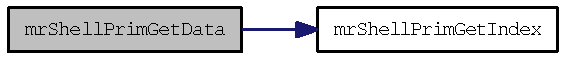
\includegraphics[width=154pt]{mrshellprim_8h_aa038cf5a29f51145c876af7fb5271d3_cgraph}
\end{center}
\end{figure}
\hypertarget{mrshellprim_8h_1e963c0f8d38ab1305d075b016de0a65}{
\index{mrshellprim.h@{mrshellprim.h}!mrShellPrimGetFloat@{mrShellPrimGetFloat}}
\index{mrShellPrimGetFloat@{mrShellPrimGetFloat}!mrshellprim.h@{mrshellprim.h}}
\subsubsection[mrShellPrimGetFloat]{\setlength{\rightskip}{0pt plus 5cm}int mr\-Shell\-Prim\-Get\-Float (\hyperlink{structArgDef__t}{TArg\-Def} $\ast$ {\em array\-Def}, const char $\ast$ {\em p\-Cmd}, float $\ast$ {\em p\-Float})}}
\label{mrshellprim_8h_1e963c0f8d38ab1305d075b016de0a65}


Get float value for an argument definition element. 

The function is only available arguments of type i\-Float. \begin{Desc}
\item[Parameters:]
\begin{description}
\item[{\em array\-Def}]argument definition array, terminated by an element of type \hyperlink{mrshellprim_8h_76a810650461f2062938ee9b82666b36a94b1781ada88507c56c4475f25fa92f}{e\-Unknown\-Type} \item[{\em p\-Cmd}]command string, both the short and the long definition are compared \item[{\em p\-Float}]data target \end{description}
\end{Desc}
\begin{Desc}
\item[Returns:]$>$=0 success, index of the element in lower 16bit; bit 16 set if this argument was found.\par
 the ARGPROC\_\-INDEX and ARGPROC\_\-EXISTS macros can be used to extract to parts\par
 neg. error code if failed\par
 -ENOENT entry not found\par
 -EBADF entry found, but of wrong type\par
 -EINVAL invalid argument\par
 -ENOSYS function not available for this type\par
 \end{Desc}


Definition at line 1040 of file mrshellprim.c.

References ARGPROC\_\-EXISTS\_\-BITSHIFT, ARGPROC\_\-FOUND, Arg\-Def\_\-t::data, e\-Float, Tagged\-Data\_\-t::Float, and mr\-Shell\-Prim\-Get\-Index().

Here is the call graph for this function:\begin{figure}[H]
\begin{center}
\leavevmode
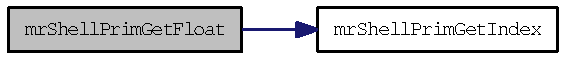
\includegraphics[width=154pt]{mrshellprim_8h_1e963c0f8d38ab1305d075b016de0a65_cgraph}
\end{center}
\end{figure}
\hypertarget{mrshellprim_8h_c08c7b1e961204b98f9b29120f043c6c}{
\index{mrshellprim.h@{mrshellprim.h}!mrShellPrimGetHex@{mrShellPrimGetHex}}
\index{mrShellPrimGetHex@{mrShellPrimGetHex}!mrshellprim.h@{mrshellprim.h}}
\subsubsection[mrShellPrimGetHex]{\setlength{\rightskip}{0pt plus 5cm}int mr\-Shell\-Prim\-Get\-Hex (\hyperlink{structArgDef__t}{TArg\-Def} $\ast$ {\em array\-Def}, const char $\ast$ {\em p\-Cmd}, unsigned int $\ast$ {\em p\-Hex})}}
\label{mrshellprim_8h_c08c7b1e961204b98f9b29120f043c6c}


Get hexadecimal value for an argument definition element. 

The function is only available for arguments of type i\-Hex \begin{Desc}
\item[Parameters:]
\begin{description}
\item[{\em array\-Def}]argument definition array, terminated by an element of type \hyperlink{mrshellprim_8h_76a810650461f2062938ee9b82666b36a94b1781ada88507c56c4475f25fa92f}{e\-Unknown\-Type} \item[{\em p\-Cmd}]command string, both the short and the long definition are compared \item[{\em p\-Hex}]data target \end{description}
\end{Desc}
\begin{Desc}
\item[Returns:]$>$=0 success, index of the element in lower 16bit; bit 16 set if this argument was found.\par
 the ARGPROC\_\-INDEX and ARGPROC\_\-EXISTS macros can be used to extract to parts\par
 neg. error code if failed\par
 -ENOENT entry not found\par
 -EBADF entry found, but of wrong type\par
 -EINVAL invalid argument\par
 -ENOSYS function not available for this type\par
 \end{Desc}


Definition at line 1070 of file mrshellprim.c.

References ARGPROC\_\-EXISTS\_\-BITSHIFT, ARGPROC\_\-FOUND, Arg\-Def\_\-t::data, e\-Hex, Tagged\-Data\_\-t::Hex, and mr\-Shell\-Prim\-Get\-Index().

Referenced by driver\-Ctrl\-Cmds(), exec\-Flash\-Erase(), and main().

Here is the call graph for this function:\begin{figure}[H]
\begin{center}
\leavevmode
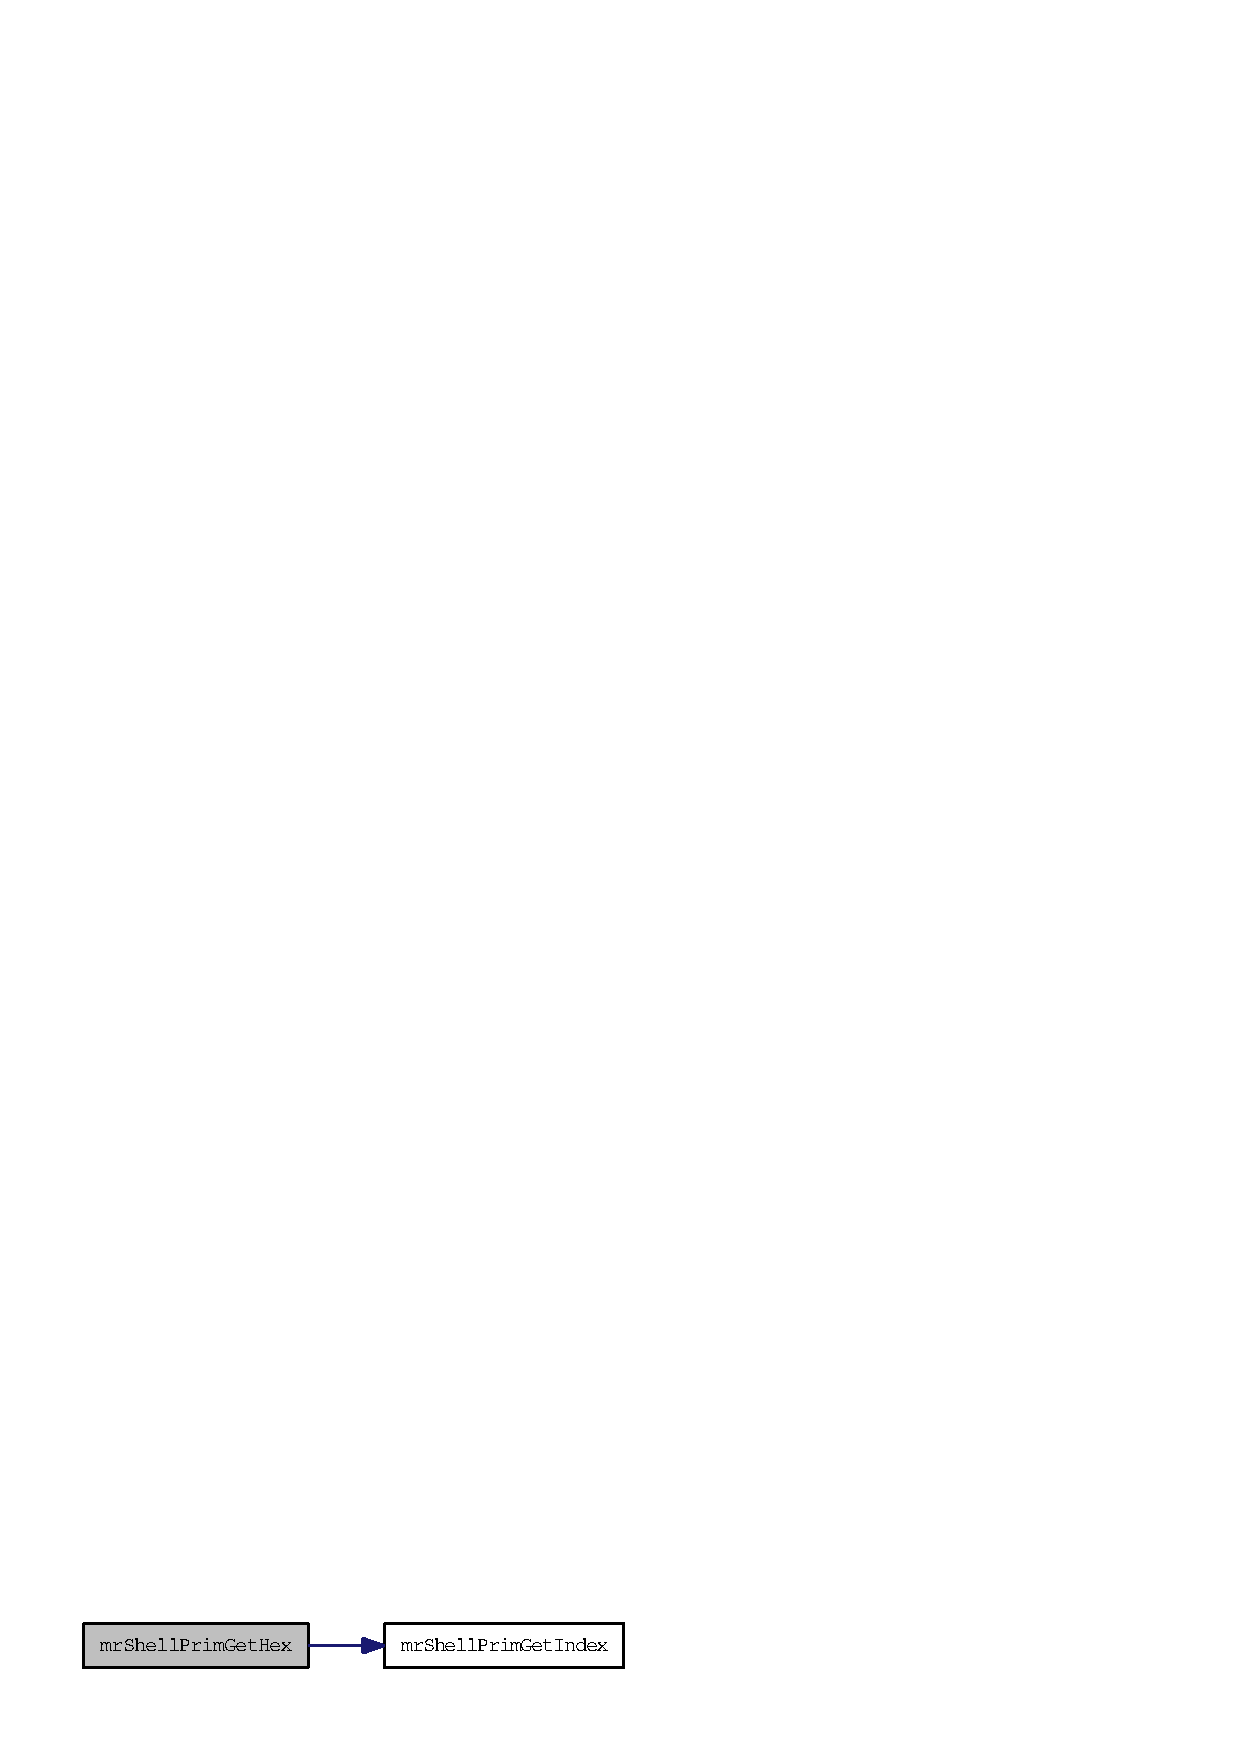
\includegraphics[width=152pt]{mrshellprim_8h_c08c7b1e961204b98f9b29120f043c6c_cgraph}
\end{center}
\end{figure}
\hypertarget{mrshellprim_8h_24d874900c59cf760f128ae366f7a72e}{
\index{mrshellprim.h@{mrshellprim.h}!mrShellPrimGetIndex@{mrShellPrimGetIndex}}
\index{mrShellPrimGetIndex@{mrShellPrimGetIndex}!mrshellprim.h@{mrshellprim.h}}
\subsubsection[mrShellPrimGetIndex]{\setlength{\rightskip}{0pt plus 5cm}int mr\-Shell\-Prim\-Get\-Index (\hyperlink{structArgDef__t}{TArg\-Def} $\ast$ {\em array\-Def}, const char $\ast$ {\em p\-Cmd}, int {\em i\-Type})}}
\label{mrshellprim_8h_24d874900c59cf760f128ae366f7a72e}


Search the argument definition for a command. 

\begin{Desc}
\item[Parameters:]
\begin{description}
\item[{\em array\-Def}]argument definition array, terminated by an element of type \hyperlink{mrshellprim_8h_76a810650461f2062938ee9b82666b36a94b1781ada88507c56c4475f25fa92f}{e\-Unknown\-Type} \item[{\em p\-Cmd}]command string, both the short and the long definition are compared \item[{\em i\-Type}]if not equal to e\-Unknown\-Type a type check is done \end{description}
\end{Desc}
\begin{Desc}
\item[Returns:]$>$=0 success, index of the element neg. error code if failed\par
 -ENOENT entry not found\par
 -EBADF entry found, but of wrong type\par
 -EINVAL invalid argument\par
 \end{Desc}


Definition at line 979 of file mrshellprim.c.

References Arg\-Def\_\-t::data, e\-Unknown\-Type, and Tagged\-Data\_\-t::type.

Referenced by mr\-Shell\-Prim\-Get\-Data(), mr\-Shell\-Prim\-Get\-Float(), mr\-Shell\-Prim\-Get\-Hex(), mr\-Shell\-Prim\-Get\-Int(), and mr\-Shell\-Prim\-Set\-Data().\hypertarget{mrshellprim_8h_8f73442602070f02c40b4b3e32ab61a3}{
\index{mrshellprim.h@{mrshellprim.h}!mrShellPrimGetInt@{mrShellPrimGetInt}}
\index{mrShellPrimGetInt@{mrShellPrimGetInt}!mrshellprim.h@{mrshellprim.h}}
\subsubsection[mrShellPrimGetInt]{\setlength{\rightskip}{0pt plus 5cm}int mr\-Shell\-Prim\-Get\-Int (\hyperlink{structArgDef__t}{TArg\-Def} $\ast$ {\em array\-Def}, const char $\ast$ {\em p\-Cmd}, int $\ast$ {\em p\-Int})}}
\label{mrshellprim_8h_8f73442602070f02c40b4b3e32ab61a3}


Get integer value for an argument definition element. 

The function is only available arguments of type i\-Integer and e\-Bool. \begin{Desc}
\item[Parameters:]
\begin{description}
\item[{\em array\-Def}]argument definition array, terminated by an element of type \hyperlink{mrshellprim_8h_76a810650461f2062938ee9b82666b36a94b1781ada88507c56c4475f25fa92f}{e\-Unknown\-Type} \item[{\em p\-Cmd}]command string, both the short and the long definition are compared \item[{\em p\-Int}]data target \end{description}
\end{Desc}
\begin{Desc}
\item[Returns:]$>$=0 success, index of the element in lower 16bit; bit 16 set if this argument was found.\par
 the ARGPROC\_\-INDEX and ARGPROC\_\-EXISTS macros can be used to extract to parts\par
 neg. error code if failed\par
 -ENOENT entry not found\par
 -EBADF entry found, but of wrong type\par
 -EINVAL invalid argument\par
 -ENOSYS function not available for this type\par
 \end{Desc}


Definition at line 1052 of file mrshellprim.c.

References ARGPROC\_\-EXISTS\_\-BITSHIFT, ARGPROC\_\-FOUND, Arg\-Def\_\-t::data, e\-Bool, e\-Integer, e\-Unknown\-Type, Tagged\-Data\_\-t::Int, mr\-Shell\-Prim\-Get\-Index(), and Tagged\-Data\_\-t::type.

Referenced by exec\-Flash\-Erase(), and main().

Here is the call graph for this function:\begin{figure}[H]
\begin{center}
\leavevmode
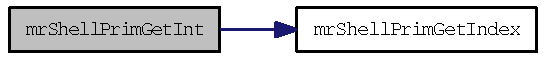
\includegraphics[width=149pt]{mrshellprim_8h_8f73442602070f02c40b4b3e32ab61a3_cgraph}
\end{center}
\end{figure}
\hypertarget{mrshellprim_8h_20b23f294fae687b7b0ad7c6483ec564}{
\index{mrshellprim.h@{mrshellprim.h}!mrShellPrimPrintDbgFlags@{mrShellPrimPrintDbgFlags}}
\index{mrShellPrimPrintDbgFlags@{mrShellPrimPrintDbgFlags}!mrshellprim.h@{mrshellprim.h}}
\subsubsection[mrShellPrimPrintDbgFlags]{\setlength{\rightskip}{0pt plus 5cm}int mr\-Shell\-Prim\-Print\-Dbg\-Flags ()}}
\label{mrshellprim_8h_20b23f294fae687b7b0ad7c6483ec564}


Print help information on the parser debug flags. 



Definition at line 966 of file mrshellprim.c.

References DBG\_\-ARGUMENT\_\-CONVERT, DBG\_\-ARGUMENT\_\-READ, DBG\_\-SCAN\_\-ARG\_\-DEF, DBG\_\-SCAN\_\-ARG\_\-DEF\_\-DETAIL, DBG\_\-SEARCH\_\-ARG\_\-DEF, and DBG\_\-SEARCH\_\-ARG\_\-DEF\_\-DETAIL.\hypertarget{mrshellprim_8h_e24662763dc15a9b4719cc0f3d98f8fc}{
\index{mrshellprim.h@{mrshellprim.h}!mrShellPrimResetVolatileFlags@{mrShellPrimResetVolatileFlags}}
\index{mrShellPrimResetVolatileFlags@{mrShellPrimResetVolatileFlags}!mrshellprim.h@{mrshellprim.h}}
\subsubsection[mrShellPrimResetVolatileFlags]{\setlength{\rightskip}{0pt plus 5cm}int mr\-Shell\-Prim\-Reset\-Volatile\-Flags (\hyperlink{structArgDef__t}{TArg\-Def} $\ast$ {\em array\-Def})}}
\label{mrshellprim_8h_e24662763dc15a9b4719cc0f3d98f8fc}


Reset volatile processing flags of the definition array. 

Reseted flags: \hyperlink{mrshellprim_8c_db27d0beb974602604e269d3efcdb71d}{ARGPROC\_\-FOUND} \begin{Desc}
\item[Parameters:]
\begin{description}
\item[{\em array\-Def}]pointer to definition array, terminated by \hyperlink{mrshellprim_8h_76a810650461f2062938ee9b82666b36a94b1781ada88507c56c4475f25fa92f}{e\-Unknown\-Type} element \end{description}
\end{Desc}
\begin{Desc}
\item[Returns:]$>$=0 success, neg. error code if failed \end{Desc}


Definition at line 1098 of file mrshellprim.c.

References ARGPROC\_\-FAILED, ARGPROC\_\-FOUND, Arg\-Def\_\-t::data, e\-Unknown\-Type, and Tagged\-Data\_\-t::type.

Referenced by Scan\-Arguments().\hypertarget{mrshellprim_8h_9f0fe9837b7198fea2f3c32bcf203ed9}{
\index{mrshellprim.h@{mrshellprim.h}!mrShellPrimSetData@{mrShellPrimSetData}}
\index{mrShellPrimSetData@{mrShellPrimSetData}!mrshellprim.h@{mrshellprim.h}}
\subsubsection[mrShellPrimSetData]{\setlength{\rightskip}{0pt plus 5cm}int mr\-Shell\-Prim\-Set\-Data (\hyperlink{structArgDef__t}{TArg\-Def} $\ast$ {\em array\-Def}, const char $\ast$ {\em p\-Cmd}, void $\ast$ {\em p\-Data}, int {\em i\-Type})}}
\label{mrshellprim_8h_9f0fe9837b7198fea2f3c32bcf203ed9}


Set data pointer for an argument definition element. 

The function is only available for other arguments than of type \hyperlink{mrshellprim_8h_76a810650461f2062938ee9b82666b36dd647739976fe8f17c25e3fe04d30eeb}{e\-Integer}, e\-Bool, i\-Float and i\-Hex. \begin{Desc}
\item[Parameters:]
\begin{description}
\item[{\em array\-Def}]argument definition array, terminated by an element of type \hyperlink{mrshellprim_8h_76a810650461f2062938ee9b82666b36a94b1781ada88507c56c4475f25fa92f}{e\-Unknown\-Type} \item[{\em p\-Cmd}]command string, both the short and the long definition are compared \item[{\em p\-Data}]void pointer to data \item[{\em i\-Type}]if not equal to e\-Unknown\-Type a type check is done \end{description}
\end{Desc}
\begin{Desc}
\item[Returns:]$>$=0 success, index of the element in lower 16bit neg. error code if failed\par
 -ENOENT entry not found\par
 -EBADF entry found, but of wrong type\par
 -EINVAL invalid argument\par
 -ENOSYS function not available for this type\par
 \end{Desc}


Definition at line 1005 of file mrshellprim.c.

References Arg\-Def\_\-t::data, e\-Bool, e\-Float, e\-Hex, e\-Integer, mr\-Shell\-Prim\-Get\-Index(), Tagged\-Data\_\-t::p\-Void, and Tagged\-Data\_\-t::type.

Here is the call graph for this function:\begin{figure}[H]
\begin{center}
\leavevmode
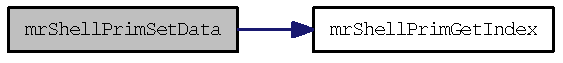
\includegraphics[width=153pt]{mrshellprim_8h_9f0fe9837b7198fea2f3c32bcf203ed9_cgraph}
\end{center}
\end{figure}
\hypertarget{mrshellprim_8h_84fd8dd7e4af266b7b6a400c0cacaea4}{
\index{mrshellprim.h@{mrshellprim.h}!mrShellPrimSetDebugFlag@{mrShellPrimSetDebugFlag}}
\index{mrShellPrimSetDebugFlag@{mrShellPrimSetDebugFlag}!mrshellprim.h@{mrshellprim.h}}
\subsubsection[mrShellPrimSetDebugFlag]{\setlength{\rightskip}{0pt plus 5cm}unsigned int mr\-Shell\-Prim\-Set\-Debug\-Flag (unsigned int {\em flag})}}
\label{mrshellprim_8h_84fd8dd7e4af266b7b6a400c0cacaea4}


Set a debug flag for the parser. 

\begin{Desc}
\item[Parameters:]
\begin{description}
\item[{\em flag}]the flag set set \end{description}
\end{Desc}
\begin{Desc}
\item[Returns:]the current value of the flags \end{Desc}


Definition at line 954 of file mrshellprim.c.

References g\_\-mr\-Shell\-Prim\-Dbg.\hypertarget{mrshellprim_8h_d50cc0ad50efa63a876cee5ef7caed9f}{
\index{mrshellprim.h@{mrshellprim.h}!PrintArgumentDefinition@{PrintArgumentDefinition}}
\index{PrintArgumentDefinition@{PrintArgumentDefinition}!mrshellprim.h@{mrshellprim.h}}
\subsubsection[PrintArgumentDefinition]{\setlength{\rightskip}{0pt plus 5cm}int Print\-Argument\-Definition (\hyperlink{structArgDef__t}{TArg\-Def} $\ast$ {\em array\-Def}, int {\em b\-All})}}
\label{mrshellprim_8h_d50cc0ad50efa63a876cee5ef7caed9f}


Print a summury on the argument definition structure. 

The type and eventually scanned values are printed out together with the flags set for the element. This is a debug feature. \begin{Desc}
\item[Parameters:]
\begin{description}
\item[{\em array\-Def}]argument definition array, terminated by an element of type \hyperlink{mrshellprim_8h_76a810650461f2062938ee9b82666b36a94b1781ada88507c56c4475f25fa92f}{e\-Unknown\-Type} \item[{\em b\-All}]\end{description}
\end{Desc}
\begin{Desc}
\item[Returns:]$>$=0 success, neg. error code if failed \end{Desc}


Definition at line 565 of file mrshellprim.c.

References ARGPROC\_\-FOUND, Arg\-Def\_\-t::data, e\-Bool, e\-Char\-Array, e\-Composite, e\-Const\-String, e\-Fct\-Arg\-Def, e\-Fct\-Composite\-Args, e\-Fct\-Float\-Args, e\-Fct\-Hex\-Args, e\-Fct\-Inclusive, e\-Fct\-Index, e\-Fct\-Integer\-Args, e\-Fct\-No\-Arg, e\-Fct\-Remaining, e\-Fct\-User\-Scan, e\-Flag, e\-Float, e\-Float\-Array, e\-Hex, e\-Hex\-Array, e\-Integer, e\-Integer\-Array, e\-Unknown\-Type, Tagged\-Data\_\-t::p\-String, and Tagged\-Data\_\-t::type.

Referenced by Scan\-Arguments().\hypertarget{mrshellprim_8h_e8ed3396fcb78ea4adce3d902b77541a}{
\index{mrshellprim.h@{mrshellprim.h}!removePrecAndTrailingSpecChars@{removePrecAndTrailingSpecChars}}
\index{removePrecAndTrailingSpecChars@{removePrecAndTrailingSpecChars}!mrshellprim.h@{mrshellprim.h}}
\subsubsection[removePrecAndTrailingSpecChars]{\setlength{\rightskip}{0pt plus 5cm}char$\ast$ remove\-Prec\-And\-Trailing\-Spec\-Chars (char $\ast$ {\em p\-Cmd})}}
\label{mrshellprim_8h_e8ed3396fcb78ea4adce3d902b77541a}


Remove preceeding and trailing special characters and blanks. 

Until now the function removes blanks at the beginning and newlines at the end.\par
 {\bf Note:} The function alters the buffer. \begin{Desc}
\item[Parameters:]
\begin{description}
\item[{\em p\-Cmd}]char buffer holding the command \end{description}
\end{Desc}
\begin{Desc}
\item[Returns:]pointer to the first non-special character of the buffer if succeeded \end{Desc}


Definition at line 44 of file mrshellprim.c.

Referenced by exec\-Batch(), and main().\hypertarget{mrshellprim_8h_e2735ecedc52b1199ecf8a208339c072}{
\index{mrshellprim.h@{mrshellprim.h}!ScanArguments@{ScanArguments}}
\index{ScanArguments@{ScanArguments}!mrshellprim.h@{mrshellprim.h}}
\subsubsection[ScanArguments]{\setlength{\rightskip}{0pt plus 5cm}int Scan\-Arguments (const char $\ast$$\ast$ {\em array\-Arg}, int {\em i\-Nof\-Args}, int {\em i\-First\-Arg\-Start}, \hyperlink{structArgDef__t}{TArg\-Def} $\ast$ {\em array\-Def}, \hyperlink{structFctMode__t}{TFct\-Mode} $\ast$ {\em p\-Mode})}}
\label{mrshellprim_8h_e2735ecedc52b1199ecf8a208339c072}


Scan a list or single string of arguments. 

with respect to the definitions of arguments as entries in the definition array, sub-functions can be called and float, decimal and hexadecimal values can be read \begin{Desc}
\item[Parameters:]
\begin{description}
\item[{\em array\-Arg}]array of argument strings \item[{\em i\-Nof\-Args}]size of the array \item[{\em i\-First\-Arg\-Start}]start of scan within the first element of the array \item[{\em p\-Separator}]a zero terminated string with additional separators, the  value is always treated as separator \item[{\em array\-Def}]an array of TArg\-Def elements, each defining a known argument type \item[{\em flags}]\end{description}
\end{Desc}
\begin{Desc}
\item[Returns:]$>$=0 successfull, offset coded\par
 bit 8-15: number of scanned elements of arg\-Array\par
 bit 0-7: offset in last processed element\par
 -EINTR if an argument with ARGDEF\_\-TERMINATE or ARGDEF\_\-BREAK was found \end{Desc}


Definition at line 692 of file mrshellprim.c.

References ARGDEF\_\-BREAK, ARGDEF\_\-DELAY\_\-EXECUTE, ARGDEF\_\-EXIT, ARGDEF\_\-RESUME, ARGDEF\_\-TERMINATE, ARGPROC\_\-FAILED, ARGPROC\_\-FOUND, call\-Command\-Handler(), DBG\_\-SCAN\_\-ARG\_\-DEF, DBG\_\-SCAN\_\-ARG\_\-DEF\_\-DETAIL, e\-Const\-String, e\-Fct\-Arg\-Def, e\-Fct\-Inclusive, Arg\-Def\_\-t::flags, Fct\-Mode\_\-t::flags, g\_\-mr\-Shell\-Prim\-Dbg, Get\-Nof\-Required\-Args(), Is\-Separator(), Arg\-Def\_\-t::l, mr\-Shell\-Prim\-Reset\-Volatile\-Flags(), Fct\-Mode\_\-t::p\-Delimiters, Print\-Argument\-Definition(), Read\-Argument(), Arg\-Def\_\-t::s, SCANMODE\_\-FORCE\_\-TERMINATION, SCANMODE\_\-PERSISTENT, SCANMODE\_\-PRINT\_\-UKWN\_\-SEQU, SCANMODE\_\-READ\_\-ONE\_\-CMD, SCANMODE\_\-SILENT, SCANMODE\_\-SKIP\_\-UKWN\_\-SEQU, SCANRET\_\-BITSHIFT\_\-INDEX, SCANRET\_\-BITSHIFT\_\-OFFSET\_\-LAST\_\-ARG, SCANRET\_\-BITSHIFT\_\-PROCESSED\_\-ARGS, SCANRET\_\-INVAL\_\-INDEX, SCANRET\_\-MASK\_\-INDEX, SCANRET\_\-MASK\_\-OFFSET\_\-LAST\_\-ARG, SCANRET\_\-MASK\_\-PROCESSED\_\-ARGS, and Search\-Def().

Referenced by call\-Command\-Handler(), execute\-Command\-Args(), main(), and Read\-Argument().

Here is the call graph for this function:\begin{figure}[H]
\begin{center}
\leavevmode
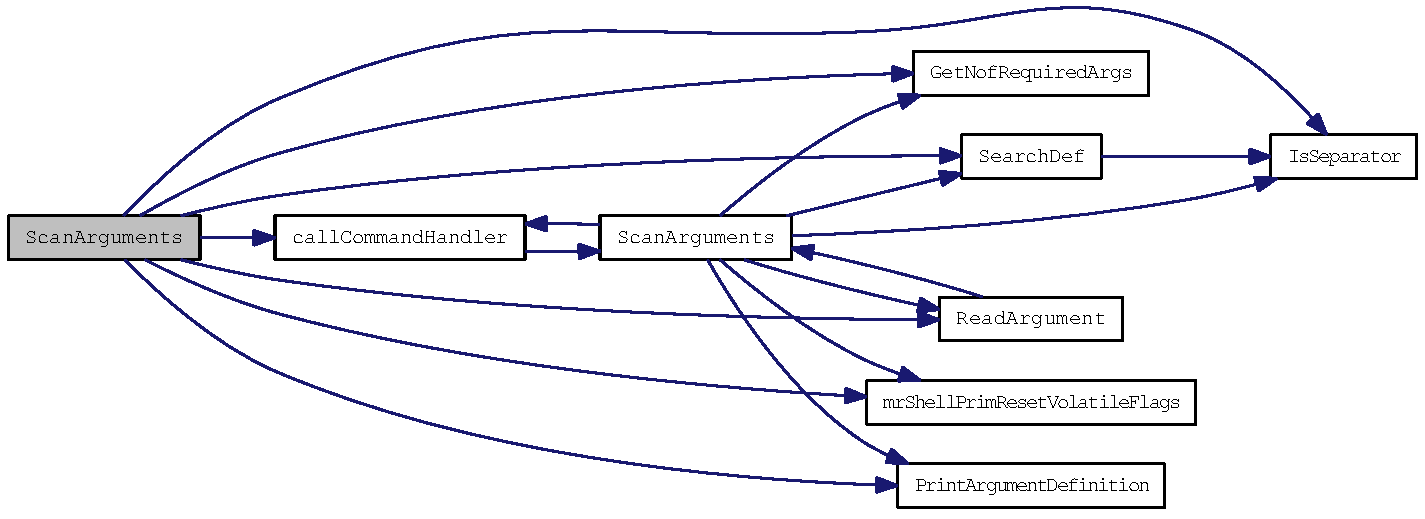
\includegraphics[width=360pt]{mrshellprim_8h_e2735ecedc52b1199ecf8a208339c072_cgraph}
\end{center}
\end{figure}
